\documentclass{llncs}

\renewcommand\floatpagefraction{.8}
\renewcommand\topfraction{.8}
\renewcommand\bottomfraction{.8}
\renewcommand\textfraction{.2}   

\renewcommand\textfloatsep{0.3cm}
% \renewcommand\baselinestretch{0.9}
\addtolength{\textheight}{0.2cm}
%% \addtolength{\textwidth}{0.1cm}

\newcommand{\sectionname}{Section}

\usepackage{xcolor}
\usepackage{listings}
\usepackage{amsmath}
\usepackage{amssymb}
\usepackage{calc}
\usepackage{rotating}
\usepackage{subfigure}
\usepackage[ruled,vlined,linesnumbered]{algorithm2e}

\usepackage{pgf}
\usepackage{tikz}

% \usepackage{electComp}
\usetikzlibrary{decorations,decorations.pathmorphing,decorations.pathreplacing}
\usetikzlibrary{arrows,automata}
\usetikzlibrary{positioning}

% \tikzstyle{loop above}=[in=75,out=105,loop]

\tikzset{
    state/.style={
      rectangle,
      rounded corners,
      draw=black, very thick,
      minimum height=2em,
      inner sep=2pt,
      text centered,
    },
}

\tikzset{
    location/.style={
      circle,
      minimum size=15pt,
      draw=black,
      text=black,
      inner sep=1.5pt
    },
}

\newcommand{\todo}[1]{{\bf \textcolor{red}{[#1]}}}

%% \newtheorem{definition}{Definition}[section]

\newcommand{\IM}{\ensuremath{\mathit{IM}}}
\newcommand{\BC}{\ensuremath{\mathit{BC}}}
\newcommand{\A}{\ensuremath{\mathcal{A}}}

\newcommand{\Reals}{\ensuremath{\mathbb{R}}}
\newcommand{\Naturals}{\ensuremath{\mathbb{N}}}
\newcommand{\Ints}{\ensuremath{\mathbb{Z}}}

% Booleens
\newcommand{\false}{{\tt false}}
\newcommand{\true}{{\tt true}}

\newcommand{\trans}[1]{\ensuremath{\overset{#1}{\rightarrow}}}
\newcommand{\Trans}[1]{\ensuremath{\overset{#1}{\Rightarrow}}}
\newcommand{\project}[1]{\ensuremath{\downarrow_{#1}}}
\newcommand{\telapse}{\ensuremath{\uparrow}}
\newcommand{\elapse}{\ensuremath{\nearrow}}
\newcommand{\valuation}{\ensuremath{\mathcal{V}}}

%% \newcommand{\qed}{\ensuremath{\square}}

\lstdefinelanguage{pha}
{
morekeywords=[1]{automaton, contr_var, synclabs, loc, while, wait, when, sync, do, goto, end, initially},
alsoletter={=},
morekeywords=[2]{==,=},
keywordstyle=[2]{\tt},
sensitive,
morecomment=[l]{//},
morecomment=[s]{/*}{*/},
morestring=[b]",
escapeinside={/*@}{@*/},
basicstyle=\sffamily\footnotesize,
breaklines=true,
xleftmargin=0.8cm,
numbers=left,
mathescape=true
}[keywords,comments,strings]

\lstdefinelanguage{imi}
{
morekeywords=[1]{automaton, var, clock, discrete, parameter, analog, synclabs, loc, while, wait, when, sync, do, goto, end, initially},
alsoletter={=},
morekeywords=[2]{==,=},
keywordstyle=[2]{\tt},
sensitive,
morecomment=[l]{//},
morecomment=[s]{/*}{*/},
morestring=[b]",
escapeinside={(@}{@)},
basicstyle=\sffamily\footnotesize,
breaklines=true,
xleftmargin=0.8cm,
numbers=left,
mathescape=true
}[keywords,comments,strings]


%%%%%%%%%%%%%%%%%%%%%%%%%%%%%%%%%%%%%%%%%%%%%%%%%%%%%%%%%%%
%%%%%%%%%%%%%%%%%%%%%%%%%%%%%%%%%%%%%%%%%%%%%%%%%%%%%%%%%%%
\begin{document}
\pagestyle{plain}

\title{Parametric Verification of Hybrid Automata Using the Inverse Method}

\author{Laurent Fribourg \and Ulrich K\"uhne}

% \institute{LSV ENS de Cachan, \\
%   61 avenue du Pr\'esident Wilson, 94235 Cachan, France \\
%   \email{\{kuehne,fribourg\}@lsv.ens-cachan.fr}
% }

\institute{LSV ENS de Cachan, 94235 Cachan, France \\
  \email{\{kuehne,fribourg\}@lsv.ens-cachan.fr}
}


\maketitle

\begin{abstract}
  Hybrid systems combine continuous and discrete behavior.  Hybrid
  Automata are a powerful formalism for the modeling and verification
  of such systems. A common problem in hybrid system verification is
  the good parameters problem, which consists in identifying a set
  of parameter valuations which guarantee a certain behavior of a
  system. Recently, a method has been presented for attacking this
  problem for Timed Automata. In this report, we show the extension of
  this methodology for hybrid automata with linear and affine
  dynamics. The method is demonstrated with a distributed temperature
  control system and several other hybrid system benchmarks from the
  literature.
\end{abstract}


%%%%%%%%%%%%%%%%%%%%%%%%%%%%%%%%%%%%%%%%%%%%%%%%%%%%%%%%%%%%%%%%%%%%%%%%%%%%
\section{Introduction} \label{sec:intro}
%% 
%% - definition hybrid systems
%% - models of hybrid systems
%% - verification problems
%% - good parameter problem
%% - inverse method
%% - cartography
%% - applications

Hybrid systems combine continuous and discrete behavior. They are
especially useful for the verification of embedded systems, as they
allow the unified modeling and the interaction of discrete control and
the continuous environment or system state such as position,
temperature or pressure. 

There are several classes of formal models for hybrid systems. In
general, there is a trade-off between the expressivity of the model
and the complexity of the algorithmic apparatus that is needed for its
formal analysis. Linear Hybrid Automata (LHA) provide a good
compromise. In contrast to more general hybrid automata models, which
allow arbitrary dynamics of the continuous state variables, LHA are
restricted to linear dynamics. This allows the use of efficient
algorithms based on convex polyhedra. Furthermore, more complex
dynamics -- like hybrid automata with affine dynamics (AHA) -- can
easily be approximated conservatively by LHA.  Although reachability
is undecidable for LHA \cite{HKPV:95}, practically relevant results
have been obtained using this formalism \cite{SMF:97,Fre:2006}.

For the modeling of embedded systems it is handy to use
\emph{parameters} either to describe uncertainties or to introduce
tuning parameters that are subject to optimization. Instead of setting
these parameters manually and then verifying the resulting concrete
system, parameterized models are used to perform automatic
\emph{parameter synthesis}. A common assumption is the existence of a
set of bad states that should never be reached. Then the parameter
synthesis can be solved by treating the parameters as additional state
variables and computing the reachable states of the parameterized
system in a standard manner~\cite{HHW:97}. However, this 
standard approach is not feasible except for
very simple cases. It is therefore essential to dynamically prune the
search space. The method presented in \cite{FJK:2008} is based on the
CEGAR approach, iteratively refining a constraint over the parameters
by discarding states that violate a given property.

While these traditional approaches to parameter synthesis are based on
the analysis of bad states or failure traces, a complementary -- or
\emph{inverse} -- method has been proposed in \cite{ACEF:2009}. It
uses a parameter instantiation that is known to guarantee a
\emph{good} behavior in order to derive a constraint on the parameters
that leads to the same behavior. While the algorithm in
\cite{ACEF:2009} is restricted to Timed Automata (TA), we present its
extension to LHA in this report. 

There are different scenarios for the application of the presented
approach. If a given parameter instantiation is known to guarantee
certain properties, the inverse method can be used to derive an
enlarged area of the parameter space that preserves these properties,
while possibly allowing for enhanced performance of the system. In the
same time, the \emph{robustness} of the parameter choice can be
proven. Since real world systems are often subject to uncertainties
wrt.~to environment conditions, it is not advisable to choose a
parameter instantiation that lies on the very edge to
malfunction. Finally, it can be used if the parameterized
\emph{verification} of a safety property is not feasible. In this
case, a pointwise verification for a set of parameter instantiations
is performed. The inverse method can then be used to obtain a measure
of \emph{coverage} of the parameter space by computing the zones of
equivalent behavior for each point. This approach is also known as
\emph{behavioral cartography} \cite{AF:2010} and will be discussed in
this report. While the natural extension of these algorithms works well
for simple LHA, it does not scale well to LHA models that approximate
more complex dynamics. Therefore, we present an enhanced algorithm
that can be applied on affine hybrid automata.

% Results on the modeling and formal verification of analog oscillator
% circuits have been reported \cite{DDM:2004,Fre:2006}. A promising
% approach is the modeling of analog circuits using hybrid automata. 

The presented algorithms are implemented in a tool called IMITATOR
(\emph{Inverse Method for Inferring Time AbstracT behaviOR})
\cite{And:2009,And:2010}. The tool has originally been developed for the
analysis of TA. The new version IMITATOR~3 implements the semantics of
LHA as presented in \sectionname~\ref{sec:lha}. The manipulation of
symbolic states is based on the polyhedral operations of the Parma
Polyhedra Library~\cite{BHZ:2009}.

The report is structured as follows. First, we will discuss related
work in \sectionname~\ref{sec:related}. In \sectionname~\ref{sec:lha},
the formal basis for the rest of the report is given. The algorithms
are introduced in \sectionname~\ref{sec:algo}. Experimental results
are discussed in the course of the presentation, using as a running
example a distributed temperature control system. More benchmarks from
the literature are treated in \sectionname~\ref{sec:results}. The
results are discussed in \sectionname~\ref{sec:disc} and the report is
concluded in
\sectionname~\ref{sec:concl}.

%%%%%%%%%%%%%%%%%%%%%%%%%%%%%%%%%%%%%%%%%%%%%%%%%%%%%%%%%%%%%%%%%%%%%%%%%%%%
\section{Related Work} \label{sec:related}

% In \cite{AKRS:2008}, a method is presented which analyzes test cases
% in the simulation of hybrid systems. The goal is very similar to our
% approach. Starting from a single simulation run of a system, it
% computes a region of initial states that do not expose new behavior
% and need not be considered as test case. But, as the method relies on
% simulation only, it cannot deal with non-determinism or uncertainties. 

The presented approach exhibits the same general differences with the
CEGAR-based approach of \cite{FJK:2008} at the LHA level as formerly
at the TA level. First, the input of CEGAR-based methods is a bad
location to be avoided while the input of our inverse method is a
good reference valuation for the parameters; second, the constraint in
CEGAR-based methods guarantees the avoidance of bad locations while the
constraint generated by the inverse method guarantees the same behavior
(in terms of discrete moves) as under the reference valuation.

Additionally, our inverse method based approach for LHA is comparable
to the symbolic analysis presented in \cite{AKRS:2008} for improving
the simulation coverage of hybrid systems.  In their work, Alur et
al.~start from an initial state $x$ and a discrete-time simulation
trajectory, and compute a constraint describing those initial states
that are guaranteed to be equivalent to $x$, where two initial states
are considered to be equivalent if the resulting trajectories contain
the same locations at each discrete step of execution.  The same kind
of constraint can be generated by our inverse method when initial
values of the continuous variables are defined using parameters. The
two methods are however methodologically different.  On the one hand,
the generalization process done by the inverse method works, using
forward analysis, by refining the current constraint over the
parameters that repeatedly discards the generated states that are
incompatible with the initial valuation of $x$; on the other hand, the
method of Alur et al.~generalizes the initial value of $x$ by
performing a backward propagation of sets of equivalent states. This
latter approach can be practically done because the system is supposed
to be {\em deterministic}, thus making easy the identification of
transitions between discrete states during the execution. Our inverse
method, in contrast, can also treat nondeterministic systems.

The approach presented in \cite{JFG+:2007} shares a similar goal,
namely identifying for single test cases a robust environment that
leads to the same qualitative behavior. Instead of using symbolic
reachability techniques, their approach is based on the stability of
the continuous dynamics. By using a bisimulation function (or
contraction map), a robust neighborhood can be constructed for each
test point. As traditional numeric simulation can be used, this makes
the technique computationally effective. But, for weakly stable
systems, a lot of test points have to be considered in order to
achieve a reasonable coverage. For some of the examples in
\cite{JFG+:2007}, we achieve better or comparable results (see Section
\ref{sec:nav}).

Note that both \cite{AKRS:2008} and \cite{JFG+:2007} only consider the
coverage of the initial states, while our approach can be applied in the
more general context of parameter synthesis.


%%%%%%%%%%%%%%%%%%%%%%%%%%%%%%%%%%%%%%%%%%%%%%%%%%%%%%%%%%%%%%%%%%%%%%%%%%%%
\section{Hybrid Automata with Parameters} \label{sec:lha}
\subsection{Basic Definitions}
In the sequel, we will refer to a set of continuous variables $X =
{x_1, \dots, x_N}$ and a set of parameters $P = {p_1, \dots, p_M}$. 
Continuous variables can take any real value. We define a valuation as
a function $w: X \rightarrow \Reals$, and the set of valuations
over variables $X$ is denoted by $\valuation(X)$. A valuation $w$ will
often be identified with the point $(w(x_1), \dots, w(x_N)) \in
\Reals^N$. A parameter valuation is a function $\pi: P \rightarrow
\Reals$ mapping the parameters to the  real numbers.

Given a set of variables $X$, a linear inequality has the form
\begin{equation}
  \sum \limits_{i=1}^{N} \alpha_i x_i \bowtie \beta,
\end{equation}
where $x_i \in X$, $\alpha_i, \beta \in \Ints$ and $\bowtie\; \in \{<,
\leq, =\}$. A convex linear constraint is a finite conjunction of
linear inequalities. The set of convex linear constraints over $X$ is
denoted by $\mathcal{L}(X)$. For a constraint $C \in \mathcal{L}(X)$
satisfied by a valuation $w \in \mathcal{V}(X)$, we write $w \models
C$. For a constraint over continuous variables and parameters $C \in
\mathcal{L}(X \cup P)$ satisfied by a valuation $w$ and a parameter
valuation $\pi$, we write $\left<w, \pi\right> \models C$. By
convention, we also write $w \models C$ for partial valuations. For
example, a valuation $w \in \mathcal{V}(X)$ is said to satisfy a
constraint $C \in \mathcal{L}(X \cup P)$ iff it can be extended with
at least one parameter valuation $\pi$ such that $\left<w, \pi\right>
\models C$.

Sometimes we will refer to a variable domain $X'$, which is obtained
by renaming the variables in $X$. Explicit renaming of variables is
denoted by the substitution operation. Here, $(C)_{[X/Y]}$ denotes the
constraint obtained by replacing in $C$ the variables of $X$ by the variables
of $Y$.

A convex linear constraint can also be interpreted as a set of points
in the space $\Reals^N$, more precisely as a convex polyhedron. We
will use these notions synonymously. In this geometric context, a
valuation satisfying a constraint is equivalent to the polyhedron
containing the corresponding point, written as $w \in C$. Also here,
for a partial valuation $w$ (i.e.~a point of a subspace of $C$), we
write $w \in C$ iff $w$ is contained in the projection of $C$ on the
variables of $w$. 

\begin{definition}\label{def:lha}
  Given a set of continuous variables $X$ and a set of parameters $P$,
  a {\em (parameterized) hybrid automaton} is a tuple $\A = (\Sigma, Q, q_0,
  I, D, \rightarrow)$, consisting of the following
  \begin{itemize}
    \item a finite set of actions $\Sigma$
    \item a finite set of locations $Q$
    \item an initial location $q_0 \in Q$ %% , where $K \subseteq I_{q_0}$
    \item a convex linear invariant $I_q \in \mathcal{L}(X \cup P)$ for each
      location $q$
    \item an activity $D_q : \Reals^n \rightarrow \Reals^n$ for each
      location $q$ 
    \item discrete transitions $q \xrightarrow{g, a, \mu} q'$, with
      guard condition $g \in \mathcal{L}(X \cup P)$, action $a \in \Sigma$
      and a jump relation $\mu \in \mathcal{L}(X \cup P \cup X')$.
  \end{itemize}
  Given a parameter constraint $K \in \mathcal{L}(P)$, the automaton
  $\A$ with the parameters restricted to $K$ is denoted by $\A(K)$.
\end{definition}

Without loss of generality,
it is assumed here that all continuous variables $x$ are initialized
with $x=0$. Arbitrary initial values can be modeled by adding a
transition with appropriate variable updates.
Parameters can be seen as additional state variables which do
not evolve in time (null activity).

The activities $D_q$ describe how the continuous variables evolve
within each location $q$. In order to obtain automata models which can
be symbolically analyzed, restrictions have to be made to these
activities. This leads to the following classes of hybrid automata.

\begin{definition}
  We define the following subclasses of hybrid automata.

  \begin{itemize}
  \item[(1)] A \emph{rectangular automaton} (RA) is a hybrid automaton,
    where in each location $q$, the time derivative $\dot{x}_i$ for
    variable $x_i$ is contained in an interval $\dot{x}_i \in \left[
      \ell_i^q, u_i^q \right]$, where $\ell_i^q, u_i^q \in \Reals$.
    
  \item[(2)] A \emph{linear hybrid automaton} (LHA) is a hybrid automaton,
    where in each location $q$, the activity is given by a convex
    linear constraint $D_q \in \mathcal{L}(\dot{X})$ over the time
    derivatives of the variables.

  \item[(3)] An \emph{affine hybrid automaton} (AHA) is a hybrid
    automaton, where in each location $q$, the activity is given by a
    convex linear constraint $D_q \in \mathcal{L}(X \cup \dot{X})$
    over the variables and the time derivatives.
  \end{itemize}
\end{definition}

Rectangular automata are a superset of timed automata (TA). The class
of timed automata can be obtained by restricting the derivatives to
$\dot{x} = 1$ and limiting the jump relations to either $x' = x$ or
$x' = 0$ (clock reset) for all variables $x \in X$. In total, the
automata models defined above form a hierarchy $TA \subset RA \subset
LHA \subset AHA$.

The reachable states of LHA can be efficiently represented by convex
polyhedra. Due to the more complex dynamics, this is not true for
AHA. In the following, we consider linear hybrid automata with
parameters. But, AHA can be approximated by LHA with arbitrary
precision by partitioning the state space, as e.g.~described
in~\cite{Fre:2008}. In \sectionname~\ref{sec:laha} it is discussed, how
these techniques can be adapted to suit our methods. In the following,
we give an example of a hybrid system, that will later on be used to
illustrate the approaches proposed in this report. 

\begin{example} \label{ex:rhb}
The \emph{room heating benchmark} (RHB) has been described in
\cite{FI:2004}. It models a distributed temperature control
system. There are $m$ movable heaters for $n > m$ rooms. The
temperature $x_i$ in each room $i$ is a continuous variable that
depends on the (constant) outside temperature $u$, the temperature of
the adjacent rooms, and whether there is an activated heater in the
room.

Depending on the relations between the temperatures measured,
the heaters will be moved. If there is no heater in room $i$, a heater
will be moved there from an adjacent room $j$, if the temperature has
reached a threshold $x_i \leq get_i$ and there is a minimum difference
of the temperatures $x_j - x_i \geq dif_i$.  Note that in contrast
with the RHB modeled in \cite{AKRS:2008}, the heater move from a room
to another one is nondeterministic, since multiple guard conditions
can be enabled simultaneously (in \cite{AKRS:2008}, the nondeterminism
is resolved by moving only the heater with the smallest index).

The dynamics of the system is given by equations of the form:
\begin{equation}\label{eq:rhb}
  \dot{x}_i = c_i h_i + b_i (u - x_i) + \sum \limits_{i\neq j} a_{i,j}(x_j - x_i)
\end{equation}
where $a_{i,j}$ are constant components of a symmetric adjacency
matrix, constants $b_i$ and $c_i$ define the influence of the outside
temperature and the effectiveness of the heater for each room $i$, and
$h_i = 1$ if there is a heater in room $i$ and $h_i = 0$ otherwise.

Here, we will study an instantiation of RHB as given in
\cite{AKRS:2008} with $n=3, m=2$, outside temperature $u=4$, the
constants $b = (0.4, 0.3, 0.4), c = (6,7,8)$. The adjacency matrix
$a_{i,j}$ is given as $\left(\begin{smallmatrix}
      0.0 \;\; & 0.5 & \;\; 0.0 \\
      0.5 \;\; & 0.0 & \;\; 0.5 \\
      0.0 \;\; & 0.5 & \;\; 0.0 \\
\end{smallmatrix}\right)$
and the thresholds are set to $get = 18$ and $dif = 1$ for all rooms.

\begin{figure}[tb]
  \centering
  \footnotesize
  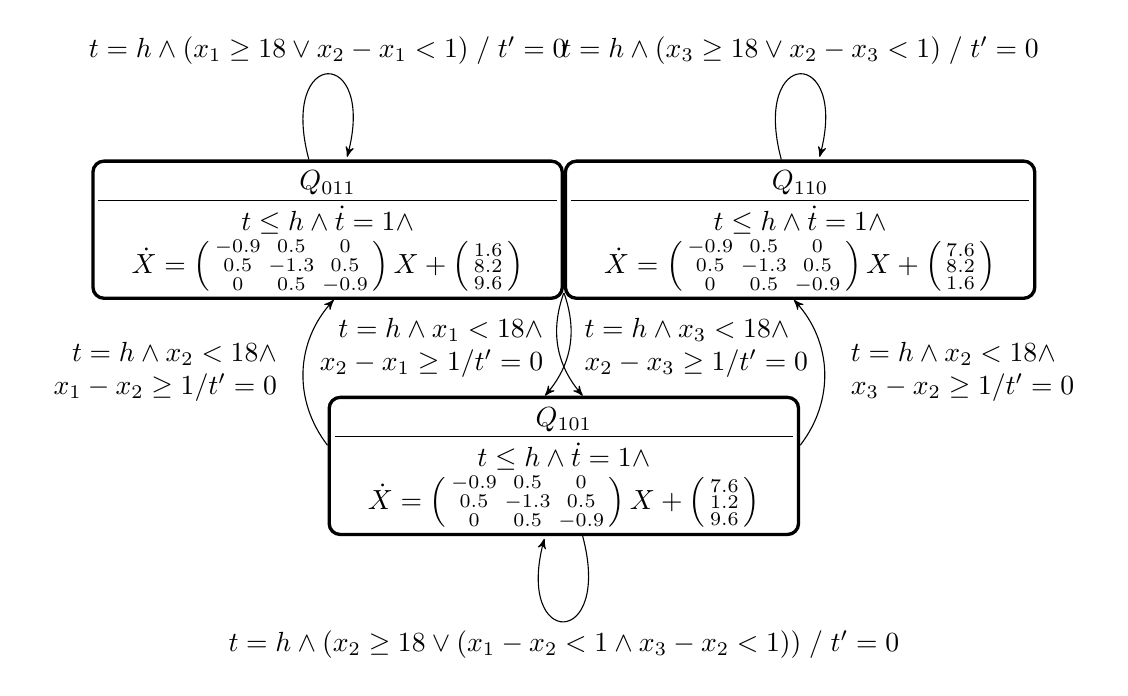
\begin{tikzpicture}[->,>=stealth']

    \node[state] (Q011) at (0,3)
    {
      \begin{tabular}{c}
        $Q_{011}$ \\
        \hline \\[-1em]
        \begin{tabular}{c}
          $t \leq h \wedge \dot{t} = 1 \wedge$ \\
          $\dot{X} = \left(\begin{smallmatrix}
              -0.9 & 0.5 & 0 \\
              0.5 & -1.3 & 0.5 \\
              0 & 0.5 & -0.9
          \end{smallmatrix} \right) X + \left(\begin{smallmatrix}
            1.6 \\ 8.2 \\ 9.6
          \end{smallmatrix}\right)$ \\
        \end{tabular}
      \end{tabular}
    };
    
    \node[state] (Q101) at (3,0)
    {
      \begin{tabular}{c}
        $Q_{101}$ \\
        \hline \\[-1em]
        \begin{tabular}{c}
          $t \leq h \wedge \dot{t} = 1 \wedge$ \\
          $\dot{X} = \left(\begin{smallmatrix}
              -0.9 & 0.5 & 0 \\
              0.5 & -1.3 & 0.5 \\
              0 & 0.5 & -0.9
            \end{smallmatrix} \right) X + \left(\begin{smallmatrix}
              7.6 \\ 1.2 \\ 9.6
            \end{smallmatrix}\right)$ \\
        \end{tabular}
      \end{tabular}
    };

    \node[state] (Q110) at (6,3)
    {
      \begin{tabular}{c}
        $Q_{110}$ \\
        \hline \\[-1em]
        \begin{tabular}{c}
          $t \leq h \wedge \dot{t} = 1 \wedge$ \\
          $\dot{X} = \left(\begin{smallmatrix}
              -0.9 & 0.5 & 0 \\
              0.5 & -1.3 & 0.5 \\
              0 & 0.5 & -0.9 
            \end{smallmatrix} \right) X + \left(\begin{smallmatrix}
              7.6 \\ 8.2 \\ 1.6
            \end{smallmatrix}\right)$ \\
        \end{tabular}
      \end{tabular}
    };

    \path

    (Q011) edge[loop above] node{$t=h \wedge (x_1 \geq 18 \vee x_2-x_1 < 1) \; / \; t' = 0$} (Q011)

    (Q110) edge[loop above] node{$t=h \wedge (x_3 \geq 18 \vee x_2-x_3 < 1) \; / \; t' = 0$} (Q110)

    (Q101) edge[loop below] node{$t=h \wedge (x_2 \geq 18 \vee (x_1-x_2 < 1 \wedge x_3-x_2 < 1))\; / \; t' = 0$} (Q101)

    (Q011)  edge[bend left=30] node[anchor=right,left]
    {
      \begin{tabular}{r}
        $t = h \wedge x_1 < 18 \wedge$ \\
        $x_2 - x_1 \geq 1 / t' = 0$
      \end{tabular}
    } (Q101)

    (Q101)  edge[bend left=40] node[anchor=right,left]
    {
      \begin{tabular}{r}
        $t = h \wedge x_2 < 18 \wedge$ \\
        $x_1 - x_2 \geq 1 / t' = 0$
      \end{tabular}
    } (Q011)

    (Q110)  edge[bend right=30] node[anchor=left,right]
    {
      \begin{tabular}{l}
        $t = h \wedge x_3 < 18 \wedge$ \\
        $x_2 - x_3 \geq 1 / t' = 0$
      \end{tabular}
    } (Q101)

    (Q101)  edge[bend right=40] node[anchor=left,right]
    {
      \begin{tabular}{l}
        $t = h \wedge x_2 < 18 \wedge$ \\
        $x_3 - x_2 \geq 1 / t' = 0$
      \end{tabular}
    } (Q110)
    
    ;
  \end{tikzpicture}
  \caption{Automaton model for room heating benchmark}\label{fig:rhbaut}
\end{figure}

The system can be modeled as an AHA, as shown in
\figurename~\ref{fig:rhbaut}. There are three control modes, corresponding
to the positions of the two heaters. The automaton has four variables,
the temperatures $X = \{x_1, x_2, x_3\}$ and a variable $t$ acting as
clock. In this example, the temperatures are sampled at a constant
rate $\frac{1}{h}$, where $h$ is a parameter of the automaton.  This
sampling scheme is used in the models of sampled-data hybrid systems
of \cite{SK:2000} and simulink/stateflow models \cite{AKRS:2008}. 

% Since the invariants associated to these modes have a disjunctive form
% (the threshold $get$ is not reached \emph{or} the difference $dif$ is
% not reached yet), they have to be modeled by multiple locations with
% convex invariants. This leads to a total of eleven locations.
\end{example}

%%%%%%%%%%%%%%%%%%%%%%%%%%%%%%%%%%%%%%%%%%%%%%%%%%%%%%%%%%%%%%%%%%%%%%%%%%%%
\subsection{Concrete semantics}
In order to obtain a concrete run of a LHA $\A(K)$, all parameters
need to be instantiated by a parameter valuation $\pi \models K$. The
instantiated model is then denoted as $\A[\pi]$. The concrete semantics
(or simulation semantics) is given by a labeled transition system
(LTS).
\begin{definition}\label{def:lts}
  A labeled transition system over a set of symbols $\Sigma$ is a
  triple $L = (S, S_0, \Rightarrow)$ with a set of states $S$, a set
  of initial states $S_0 \subseteq S$ and a transition relation
  $\Rightarrow \; \subseteq S \times \Sigma \times S$. We write $s
  \Trans{a} s'$ for $(s, a, s') \in \Rightarrow$. A run of length $m$
  is a finite alternating sequence of states and symbols of the form
  $s_0 \Trans{a_0} s_1 \Trans{a_1} \dots \Trans{a_{m-1}} s_m$, where
  $s_0 \in S_0$. A state $s_m$ is reachable if it is the last state of
  some run $R$.
\end{definition}

\begin{definition}\label{def:csem}
  The concrete semantics of an LHA $\A[\pi]$ is given by the
  LTS $L_H = (S, S_0, \Rightarrow)$ with
  \begin{itemize}
    \item states $S = \{ (q,w) \in Q \times \valuation(X) \mid \left< w, \pi \right> \models I_q \}$
    \item initial states $S_0 = \{(q_0, w) \mid \left<w, \pi \right> \models I_{q_0} \wedge \exists v, t: w = t \cdot v, t \in \Reals_{+}, v \in D_{q_0} \}$
    \item discrete transitions $(q,w) \trans{a} (q', w')$ if \\ $\exists g,\mu: q \xrightarrow{g, a, \mu} q'$ and $\left<w,\pi\right> \models g$ and $\left< w, w', \pi\right> \models \mu$
    \item delay transitions $(q,w) \trans{t} (q,w')$ if \\ $\exists v \in D_q: w' = w + t \cdot v$
    \item transitions $(q,w) \Trans{a} (q',w')$ if \\ $\exists t,w'': (q,w) \trans{a} (q',w'') \trans{t} (q',w')$
  \end{itemize}
%%  \todo{Check the initial states: do we have to instantiate also the
%%    continuous variables? Or re-introduce $\phi_0$ for this purpose?}
\end{definition}

The valuations of the initial states are obtained by letting time
elapse from the initial valuation $\bigwedge_{i = 1}^{N} x_i = 0$, while
still satisfying the invariant of $q_0$. Finally, we define the notion
of traces and their equivalence. A trace is obtained by projecting a
run on the locations:

\begin{definition}
  For a LHA $\A$, the \emph{trace associated to a concrete run}
  $(q_0, w_0) \Trans{a_0} \dots \Trans{a_{m-1}} (q_m, w_m)$ of
  $\A[\pi]$ is the alternating sequence of locations and actions 
$q_0 \Trans{a_0} \dots \Trans{a_{m-1}} q_m$.
\end{definition}
\begin{definition}
  Given a LHA $\A$ and two parameter instantiations $\pi_1$ and $\pi_2$,
  if the set of traces corresponding to the semantics of
$\A[\pi_1]$ is equal to to the set of traces corresponding to the semantics
of $\A[\pi_2]$, then  $\A[\pi_1]$ and $\A[\pi_2]$
  are said to be \emph{trace equivalent}. 
\end{definition}


%%%%%%%%%%%%%%%%%%%%%%%%%%%%%%%%%%%%%%%%%%%%%%%%%%%%%%%%%%%%%%%%%%%%%%%%%%%%
\subsection{Symbolic semantics}
The symbolic semantics of a LHA $\A(K)$ are defined at the level of
constraints. A symbolic state is a pair $(q,C)$ of a location $q$ and
a constraint $C$ over variables and parameters. The corresponding
operations are therefore performed on convex polyhedra rather than on
concrete valuations. One necessary operation is the progress of time
within a symbolic state, modeled by the \emph{time-elapse} operation.

\begin{definition}\label{def:telapse_qt}
Given a symbolic state $(q,C)$, the states reached by letting $t$ time
units elapse, while respecting the invariant of $q$, are characterized
as follows
\begin{equation*}
  w' \in C \telapse_{q}^{t} \quad \text{iff} \quad \exists w \in C, v \in D_q: w' = w + t\cdot v \wedge w' \in I_q
\end{equation*}
\end{definition}

Note that due to the convexity of the invariants, if $C \subseteq I_q$
and $C\telapse_{q}^{t} \subseteq I_q$, then also $\forall t' \in
[0,t]: C\telapse_{q}^{t'} \subseteq I_q$. To obtain any state
respecting the invariant that is reached by letting some time elapse,
we use the closure of the above operation.

\begin{definition}\label{def:telapse}
Given a symbolic state $(q,C)$, the closure of the time-elapse
operation is defined as follows
\begin{equation*}
  w' \in C \telapse_{q} \quad \text{iff} \quad \exists t \in \Reals_+: w' \in C \telapse_{q}^{t}
\end{equation*}
\end{definition}

Note that this operator preserves the convexity of $C$.
Furthermore, the operator $C \project{X}$ denotes the projection of the
constraint $C$ on the variables in $X$, which is performed by
existential quantification (e.g.~using Fourier-Motzkin elimination) of
the variables not contained in $X$. Based on these definitions, the
symbolic semantics of a LHA $\A(K)$ is given by a labeled transition
system (LTS) as follows.

\begin{definition}\label{def:ssem}
  The symbolic semantics of LHA $\A(K)$ is a LTS with
  \begin{itemize}
  \item states $S = \{ (q,C) \in Q \times \mathcal{L}(X \cup P) \mid C \subseteq I_q \}$
  \item initial state $s_0 = (q_0, C_0)$ with $C_0 =  K \wedge [\bigwedge_{i=1}^N x_i=0] \telapse_{q_0}$
  \item discrete transitions $(q,C) \trans{a} (q',C')$ if exists $q \trans{a,g,\mu} q'$ and \\
    $C' = \big( \left[ C(X) \wedge g(X) \wedge \mu(X,X') \right]
    \project{X'} \wedge I_{q'}(X') \big)_{[X'/X]}$
  \item delay transitions $(q,C) \trans{t} (q,C')$ with \\
    $C' = C \telapse_q^t$
  \item transitions $(q,C) \overset{a}{\Rightarrow} (q',C')$ if \\
    $\exists t,C'': (q,C) \trans{a} (q',C'') \trans{t} (q',C')$, or as a closed formula:\\
    $C' = \big( \left[ \left[ C(X) \wedge g(X) \wedge \mu(X,X') \right] \project{X'} \wedge I_{q'}(X') \right] \telapse_{q'} \big)_{[X'/X]}$
  \end{itemize}
\end{definition}

% The somewhat nice algorithmic properties of LHA are based on the fact
% that the convexity of the involved constraints is preserved under the
% transition relation. While this is trivial for most of the operations,
% it is not obvious for the time-elapse operator.

% \begin{lemma}\label{lem:elapse}
%   For a symbolic state $(q,C)$, the time-elapse operation $C
%   \telapse_q$ can be effectively computed and it preserves the
%   linear convexity of $C$.
% \end{lemma}
% %
% A proof based on operations on polyhedra can be found in
% \cite{HPR:97}.

Analogously to the concrete semantics, the {\em trace of a symbolic run}
$(q_0, C_0) \Trans{a_0} \dots \Trans{a_{m-1}} (q_m, C_m)$ is obtained
by projecting the symbolic states to the locations,
which gives: $q_0
\Trans{a_0} \dots \Trans{a_{m-1}} q_m$. Two runs (concrete or
symbolic) are said to be {\em equivalent}, if their corresponding traces are
equal.

The set of states reachable from any state in a set $S$ in exactly $i$
steps is denoted as $Post^{i}_{\A(K)}(S)$. More formally,
$Post^{i}_{\A(k)} = \{s' \mid \exists s \in S: s \Trans{a_{0}} \dots
  \Trans{a_{i-1}} s'\}$. Likewise, the set of all reachable states from
$S$ is defined as $Post^{*}_{\A(K)}(S) = \bigcup_{i\geq
  0}Post^{i}_{\A(K)}$. The reachable states of $\A(K)$ are defined as
$Reach_{\A(K)} = Post^{*}_{\A(K)}(\{s_0\})$, where $s_0$ is the
initial state of $\A(K)$.


%%%%%%%%%%%%%%%%%%%%%%%%%%%%%%%%%%%%%%%%%%%%%%%%%%%%%%%%%%%%%%%%%%%%%%%%%%%%
\subsection{Relation between concrete and symbolic semantics}
The concrete semantics captures every single run that is admissible in
an automaton. While it is easy to see its relation to the automaton,
it cannot be used for the formal verification of systems modeled as
LHA, since the number of concrete runs is almost always
infinite. Instead, the symbolic semantics allows for a more abstract
view on the system by capturing sets of runs. It is based on linear
constraints which can be interpreted as convex sets of valuations. For
the manipulation of such constraints, there exist geometric algorithms
operating on convex polyhedra \cite{CH:78,HPR:97,BHZ:2009}.

More precisely, it can be shown that every concrete run can be
simulated by a symbolic run and vice versa. The following statements
are motivated by \cite{HRSV:2001}. Their proofs can easily be adapted
to the LHA model. First, we state again the preservation of convexity
by the time-elapse operation.

\begin{lemma}\label{lem:elapse}
  For a symbolic state $(q,C)$, the time-elapse operation $C
  \telapse_q$ can be effectively computed and it preserves the
  linear convexity of $C$.
\end{lemma}
%
A proof based on operations on polyhedra can be found in
\cite{HPR:97}.

\begin{lemma}\label{lem:init_sc}
  For the initial state $(q_0, C_0)$ of the symbolic semantics of a
  LHA $\A(K)$, there is an initial state $(q_0, w_0)$ in the
  concrete semantics of $\A[\pi]$ for each parameter
  valuation $\pi$ and each valuation $w_0$ with $\left<w_0, \pi\right>
  \models C_0$.
\end{lemma}

\begin{proof}
  According to Definition \ref{def:ssem}, we show that each valuation
  $w$ with $\left<w, \pi\right> \models K \wedge [\bigwedge_{i=1}^N
  x_i=0]\telapse_{q_0}$ corresponds to an initial state $(q,w)$
  according to Definition \ref{def:csem}.  By definition of the
  time-elapse operation, we have $w \in [\bigwedge_{i=1}^N x=0]
  \telapse_{q_0} \Rightarrow \exists t \in \Reals_+, v \in D_{q_0}: w
  = t \cdot v$. As also $\left<w, \pi\right> \models I_{q_0}$, this
  completes the proof.  \qed
\end{proof}

\begin{lemma}\label{lem:step_sc}
  For each step $(q,C) \Trans{a} (q',C')$ in the symbolic semantics of
  $\A(K)$ and 
each valuation $w'$ and
  $\pi$ with $\left<w',\pi\right> \models C'$,
 there is a step $(q,w) \Trans{a} (q',w')$ in the
  concrete semantics of $\A[\pi]$ for some valuation
$w$ with $\left<w,\pi\right> \models C$.
\end{lemma}

\begin{proof}
  We decompose the proof for the transition $(q,C) \Trans{a} (q', C')$
  into the steps $(q,C) \trans{a} (q',C'') \trans{t} (q', C')$.

  For the delay transition $(q', C'') \trans{t} (q', C')$, we have $C'
  = C''\telapse_{q'}$. Since $(q',C'')$ and $(q',C')$ are states in
  the symbolic semantics, we have $C'' \subseteq I_{q'}$ and $C'
  \subseteq I_{q'}$. Following Lemma \ref{lem:elapse},
  $C''\telapse_{q'}$ is convex and also $C'' \subseteq
  C''\telapse_{q'}$. Thus, if $\left<w',\pi\right> \models C'$, this
  implies $\left<w',\pi\right> \models I_{q'}$ and there exist $w''
  \in C'', v \in D_{q'}, t \in \Reals_+$ such that $w'$ can be
  reached by letting time elapse to $w' = w'' + t \cdot v$. It follows
  that $\left<w'',\pi\right> \models I_{q'}$. Thus,
  $(q', w'')$ is a state in the concrete semantics with $(q', w'')
  \trans{t} (q', w')$ and $\left<w'', \pi\right> \models C''$.

  According to Definition \ref{def:ssem}, for step $(q,C) \Trans{a}
  (q',C')$ there exists a discrete transition in the automaton
  $\A$ with $q \xrightarrow{g,a,\mu} q'$. We have $(q,C)
  \trans{a} (q',C'')$ and thus $C''(X') = \left[ C(X) \wedge g(X)
    \wedge \mu(X,X')\right] \project{X'} \wedge I_{q'}(X')$. As shown
  above, there exists a valuation $w''$ with $\left<w'', \pi\right>
  \models C''$. Since $C'' \neq \false$, we can conclude that $\exists
  w: \left<w,\pi\right> \models C \; \wedge \; \left<w,\pi\right>
  \models g \; \wedge \left<w, w'',\pi\right> \models
  \mu$. Since $C \subseteq I_{q}$, the state $(q,w)$ is a state in the
  concrete semantics. This gives us the concrete discrete
  transition $(q,w) \trans{a} (q',w'')$ according to Definition
  \ref{def:csem}. Together with the delay transition, we have
  $(q,w)\trans{a}(q',w'')\trans{t}(q',w')$ and thus
  $(q,w)\Trans{a}(q',w')$.
 \qed
\end{proof}

This allows us now to state the correspondence of symbolic and
concrete runs:
\begin{proposition}\label{prop:run_sc}
  For each symbolic run of $\A(K)$ reaching $(q,C)$, for each
  parameter valuation $\pi$ and clock valuation $w$ with $\left< w,
    \pi \right> \models C$, there is an equivalent concrete run of
  $\A[\pi]$ reaching $(q,w)$.
\end{proposition}

\begin{proof}
  By induction over the length of the run. The base case -- a run with
  0 transitions -- directly follows from Lemma \ref{lem:init_sc}.

  By induction hypothesis, we have a symbolic run ending in $(q,C)$
  and a corresponding concrete run ending in $(q,w)$ with $w \models
  C$. For the induction step, we assume that we have an extended
  symbolic run ending with a transition $(q, C) \Trans{a} (q', C')$
  and $\left<w', \pi\right> \models C'$. Following Lemma
  \ref{lem:step_sc}, there exists a concrete step $(q, w) \Trans{a}
  (q', w')$. The concrete run can be therefore be extended by the step
  $(q,w) \Trans{a} (q',w')$, resulting in the required concrete run.
  \qed
\end{proof}

Similarly, the converse direction can be shown. 

\begin{lemma}\label{lem:init_cs}
  Given an initial state $(q_0,w)$ of the concrete semantics of
  $\A[\pi]$, there exists an initial state $(q_0,C)$ of the
  symbolic semantics of $\A(K)$ for some parameter constraint
  $K$ such that $\left<w, \pi\right> \models C$.
\end{lemma}

\begin{proof}
  For the concrete initial state $(q_0, w)$, we have
  $\left<w,\pi\right> \models I_{q_0}$ and $\exists v, t:
  w = t \cdot v, t \in \Reals_+, v \in D_{q_0}$. According to Definition
  \ref{def:telapse}, this implies that $\left<w, \pi\right>
  \models [\bigwedge_{i=1}^N x_i=0] \telapse_{q_0}$. Furthermore, choosing any $K$ with
  $\pi \models K$, we also have $\left<w, \pi\right> \models
  K$. Finally, as $\left<w, \pi\right> \models I_{q_0}$, this proves
  that $(q_0, C)$ with $C = K \wedge [\bigwedge_{i=1}^N x_i=0]\telapse_{q_0}$ is an
  initial state in the symbolic semantics of $\A(K)$.
\end{proof}

\begin{proposition}\label{prop:run_cs}
  For each parameter valuation $\pi \models K$ and valuation
  $w$, if there is a concrete run of $\A[\pi]$, reaching $(q,
  w)$, then there is an equivalent symbolic run of
  $\A(K)$, reaching state $(q, C)$ for some $C$ such that $\left<w, \pi\right>
  \models C$.
\end{proposition}

\begin{proof}
  By induction over the length of the run. The base case -- again a
  run with 0 transitions -- follows from Lemma \ref{lem:init_cs}.

  By induction hypothesis, there exists a concrete run of $\A[\pi]$
  ending in $(q,w)$ and a corresponding symbolic run for some $\A(K)$
  with $\pi \models K$ ending in a state $(q,C$) with
  $\left<w,\pi\right> \models C$.  For the induction step, we assume an
  extended concrete run of $\A[\pi]$, ending with the step $(q,w) \Trans{a}
  (q',w')$.

  The considered concrete step $(q,w) \Trans{a} (q',w')$ consists of
  the two steps $(q,w) \trans{a} (q',w'') \trans{t} (q',w')$. By
  Definition \ref{def:csem}, there exists a transition $q
  \xrightarrow{g,a,\mu} q'$ in the automaton $\A$ such that
  $\left<w, \pi\right> \models g$ and $\left<w,w'',\pi\right> \models
  \mu$. Since also $\left<w,\pi\right> \models I_q$ and
  $\left<w',\pi\right> \models I_{q'}$, it follows that there exist
  $C,C''$ with $\left<w, \pi\right> \models C$ and
  $\left<w'',\pi\right> \models C''$ such that $C''(X') = \left[ C(X)
    \wedge g(X) \wedge \mu(X,X') \right] \project{X'} \wedge I_{q'}$
  and $C \subseteq I_q$. Thus, $(q,C)$ and $(q',C'')$ are states in
  the symbolic semantics and $(q,C) \trans{a} (q',C'')$.

  For the concrete state $(q', w'')$ with the delay transition $(q',
  w'') \trans{t} (q',w')$, following Definition \ref{def:csem} there
  exist $v \in D_{q'}, t \in \Reals_+$ such that $w' = w'' + t
  \cdot v$. And thus, since $\left<w'', \pi\right> \models C''$ and
  $\left<w', \pi\right> \models I_{q'}$, it follows that $\left<w',
    \pi\right> \models C'' \telapse_{q'}$. Following Definition
  \ref{def:ssem}, we have a symbolic delay transition $(q', C'')
  \trans{t} (q', C')$. Together with the discrete transition, we can
  finally extend the assumed path with the step $(q, C) \Trans{a} (q',
  C')$, ending in symbolic state $(q', C')$ with $\left<w', \pi\right>
  \models C'$.  \qed
\end{proof}

Note that the symbolic semantics of $\A(K)$ can contain more traces
than any single concrete semantics of $\A[\pi]$ for some $\pi \models
K$. In general, if there is a parameter valuation $\pi$ and a
parameter constraint $K$, such that for all reachable states $(q,C)$
of $\A(K)$, it holds that $\pi \models C$, then $\A(K)$ and $\A[\pi]$
are trace equivalent.

Furthermore, note that during a run of $\A(K)$, the parameter
constraints associated to the reachable states can only get stronger,
since the parameters do not evolve under the time elapse operation,
and can only be further constrained by invariants or guard
conditions. This gives rise to the following observation.

\begin{lemma}\label{lem:narrow}
  For any reachable state $(q,C) \in Reach_{\A(K)}$, it holds that
  $(\exists X: C) \subseteq K$. This implies that for each parameter
  valuation $\pi \models C$, also $\pi \models K$. 
\end{lemma}

The lemma follows directly from the definition of the symbolic
semantics. We say that a state $(q,C)$ is \emph{compatible} with a
parameter valuation $\pi$, or just \emph{$\pi$-compatible}, if $\pi
\models C$. Conversely, it is \emph{$\pi$-incompatible} if $\pi
\not\models C$.

These observations are the basis for the \emph{Inverse Method}, which
is described in the following section.


%%%%%%%%%%%%%%%%%%%%%%%%%%%%%%%%%%%%%%%%%%%%%%%%%%%%%%%%%%%%%%%%%%%%%%%%%%%%
\section{Algorithm}\label{sec:algo}
\subsection{Inverse Method}

The Inverse Method for LHA attacks the good parameters problem by
generalizing a parameter valuation $\pi$ that is known to guarantee a
good behavior. Thereby, the valuation $\pi$ is relaxed to a constraint
$K$ such that the \emph{discrete behavior} -- i.e.~the set of
traces -- of $\A[\pi]$ and $\A(K)$ is identical. The algorithm has
first been described for parametric timed automata
in~\cite{ACEF:2009}, and has been applied for the synthesis of timing
constraints for memory circuits \cite{And:2009}.

\begin{algorithm}[tb]
  \SetKwInOut{Input}{input}\SetKwInOut{Output}{output}

  \Input{Parametric linear hybrid automaton $\A$} %%  of initial state $s_0 = (q_0, K_0)$} %% FIXME: what is this for?
  \Input{Valuation $\pi$ of the parameters}
  
  \Output{Constraint $K_0$ on the parameters}
  
  \BlankLine

  $ i \leftarrow 0\,;\ \  K \leftarrow \true \,; \ \ S \leftarrow \{ s_0 \} $


  % WHILE TRUE DO
  \While{\true}{
    % WHILE INCOMPATIBLE DO
    \While{there are $\pi$-incompatible states in $S$}
    {
      Select a $\pi$-incompatible state $(q, C)$ of $S$ (i.e., s.t. $\pi \not\models C$) \label{IM:select_state} \;
		
      Select a $\pi$-incompatible inequality $J$ in $(\exists X : C)$ (i.e., s.t. $\pi \not\models J$) \label{IM:select_conjunct}\;

      $K \leftarrow K \wedge\neg J $ \;
      $S \leftarrow \bigcup^i_{j = 0} \mathit{Post}^j_{\A(K)}(\{ s_0 \})$ \; \label{IM:post_update}
    } % ENDWHILE
    % \tcp*{$S$ is $\pi$-compatible}
	
    % IF
    % \lIf{$\mathit{Post}_{\A(K)}(S) = \emptyset$}
    \lIf{$\mathit{Post}_{\A(K)}(S) \sqsubseteq S $}{\Return{$K_0 \leftarrow \bigcap_{(q, C) \in S} (\exists X :C)$}} \label{IM:terminate}

    $i \leftarrow i+1$ \;
    $S \leftarrow S \cup \mathit{Post}_{\A(K)}(S)$
%%    \tcp*{$S = \bigcup^i_{j = 0} \mathit{Post}^j_{\A(K)}(\{ s_0 \})$}
    
  } % ENDWHILE

  % RETURN
  \caption{$\IM(\A, \pi)$}\label{algo:IM}
\end{algorithm}

Algorithm~\ref{algo:IM} describes the Inverse Method for LHA. The
overall structure is similar to a reachability analysis. In the main
loop, the reachable states with increasing depth $i$ are computed. In
parallel, the constraint $K$ is derived. It is initialized with
$\true$. Each time a $\pi$-incompatible state $(q,C)$ is reached, $K$
is refined such that the incompatible state is unreachable for
$\A(K)$. If $C$ is $\pi$-incompatible, then there must be at least one
inequality $J$ in its projection on the parameters ($\exists X:C$),
which is incompatible with $\pi$. The algorithm selects one such
inequality and adds its negation $\neg J$ to the constraint
$K$. Before continuing with the search, the reachable states found so
far are updated to comply with the new constraint $K$ (line
\ref{IM:post_update}). If there are no more $\pi$-incompatible states,
then $i$ is increased and the loop continues.

The algorithm stops as soon as no new states are found (line
\ref{IM:terminate}). The output of the algorithm is then a parameter
constraint $K_0$, obtained as the intersection of the constraints
associated with the reachable states.  The resulting constraint can be
characterized as follows.

\begin{proposition}
  Suppose that the algorithm $\IM(\A, \pi_0, k)$ terminates with the
  output $K_0$. Then the following holds:
  \begin{itemize}
  \item $\pi_0 \models K_0$
  \item For all $\pi \models K_0$, $\A[\pi_0]$
    and $\A[\pi]$ are trace equivalent, i.e.~the sets of traces are identical 
  \end{itemize}
\end{proposition}
\begin{proof}
  Based on Lemma~\ref{lem:narrow} and Propositions~\ref{prop:run_sc}
  and \ref{prop:run_cs}, the proof in \cite{ACEF:2009} can be extended
  for LHA in a straightforward manner. \qed
\end{proof}

In other words, we obtain a (convex) constraint including the initial
point $\pi_0$, that describes a set of parameter valuations for which
the same set of traces is observable. In particular, if $\A[\pi_0]$ is
known to avoid a set of (bad) locations for $\pi_0$, so will $\A[\pi]$
for any $\pi \models K_0$.

Note that the intersection in line~\ref{IM:terminate} is necessary --
rather than just returning $K$ -- in order to guarantee the
equivalence of the traces. Without this operation, it is possible that
the symbolic semantics of $\A(K)$ contains additional traces caused by
deadlocks that do not occur in $\A[\pi_0]$. For more details, refer to
\cite{ACEF:2009}. 

The algorithm $\IM$ is not guaranteed to terminate
\footnote{Termination of such a general reachability-based procedure
  cannot be guaranteed due to undecidability of reachability for TA
  with parameters and LHA \cite{HKPV:95}}.  Note also that the
presented algorithm involves nondeterminism. In
Algorithm~\ref{algo:IM} in lines \ref{IM:select_state} and
\ref{IM:select_conjunct}, one can possibly choose among several
incompatible states and inequalities. This may lead to different --
nevertheless correct -- results. This implies in particular that the
resulting constraint $K_0$ is not maximal in general. In order to
further explore a hybrid system, the \emph{behavioral cartography} can
be applied, which is described in the next section. Before, we give
a case study of the application of the inverse method.

\begin{example} \label{ex:rhb2}
  In order to enable the application of the inverse method as
  described above to the RHB from example \ref{ex:rhb}, the AHA
  automaton is converted to a LHA.  This is done using the {\em
    phase-portrait} approximation described in \cite{HW:96}. The space
  is partitioned into regions, and within each region, the activity
  field is overapproximated using linear sets of activity vectors.
  For each region $R$ delimiting a portion of the partitioned state
  space, the activities are statically overapproximated as
  \begin{equation}
    \dot{x}_i \in \left[ min \{f_i(x) \mid x \in R \}, max \{f_i(x) \mid x \in R \} \right]
  \end{equation}
  where $f_i(x)$ corresponds to the right-hand side in \eqref{eq:rhb}.
  The approximation can be made arbitrarily accurate by approximating
  over suitably small regions of the state space. Here, each region
  $R$ corresponds to a unit cube (of size 1 degree Celsius) in the
  dimensions $x1,x2,x3$.

  \begin{figure}[tb]
  \centering
  \subfigure[Starting from a single point]{
    \includegraphics[width=3.5cm]{images/point_x1} \; 
    \includegraphics[width=3.5cm]{images/point_x2} \;
    \includegraphics[width=3.5cm]{images/point_x3}
    \label{fig:plot_point}
  }
  \subfigure[Starting from a tile synthesized by the Inverse Method]{
    \includegraphics[width=3.5cm]{images/plot_t_x1} \; 
    \includegraphics[width=3.5cm]{images/plot_t_x2} \;
    \includegraphics[width=3.5cm]{images/plot_t_x3}
    \label{fig:plot_zone}
  } 
  \caption{Reachable states for room heating benchmark}\label{fig:plot_rhb}
\end{figure}

  The inverse method considers only the discrete behavior of a
  system. It is thus well suited for qualitative properties that
  address the switching of discrete states.  Such properties have been
  considered in \cite{FI:2004}, e.g.:
  \begin{itemize}
  \item All rooms eventually get a heater
  \item In all rooms there will eventually be no heater
  \end{itemize}
  In our model, we will use the inverse method to show a slightly
  weaker property, a bounded liveness property that is expressible as
  a safety condition as follows.  
  \begin{description}
  \item{\textit{Prop1:}} At least one of the heaters will be moved within a
    given time interval $[0, t_{max}]$ with $t_{max} = \frac{1}{2}$
    and a sampling time $h=\frac{1}{10}$.
  \end{description}
  The upper bound $t_{max}$ plays here the role of the maximal number
  of discrete transitions that are used in the method of
  \cite{AKRS:2008}. In the automaton model, a violation of the
  property is modeled by a transition to a location $q_{bad}$. To
  check the property for varying initial conditions, we add the
  parameters $a_1, a_2, a_3$ and constrain the initial state with
  $x_1=a_1 \wedge x_2=a_2 \wedge x_3=a3$.
  
  The property can be checked by standard reachability analysis
  starting from a single point\footnote{In a first attempt, we checked
    this property using standard parametric reachability analysis. We
    considered the initial state wrt.~the temperatures $(x1,x2,x3)$ to
    be within the rectangular region $[16,18]^3$. But, no result could
    be obtained in this way due to the large state space.} $(a_1, a_2,
  a_3)$.  Starting from the initial point $(a_1, a_2,
  a_3)=(18,17,18)$, the reachable states for the variables $x_1$,
  $x_2$ and $x_3$ are shown in \figurename~\ref{fig:plot_point}. The
  bad location is not reached from this point. Using the Inverse
  Method (Algorithm~\ref{algo:IM}), the initial point can be
  generalized to a larger region around the starting point $(18, 17,
  18)$, resulting in the constraint
  \begin{equation*}
    a_1 \geq a_2 + \tfrac{181}{200} \, \wedge \, a_1 < \tfrac{a_3}{2} + \tfrac{37}{4} \, \wedge \, a_2 > \tfrac{3381}{200} \, \wedge 
    \, a_2 < \tfrac{35}{2} \, \wedge \,  a_3 > \tfrac{35}{2} \, \wedge \, a_3 < \tfrac{456}{25}.
  \end{equation*}

  The symbolic runs starting from this enlarged initial region are
  depicted in \figurename~\ref{fig:plot_zone}.  The sets of traces of the
  two figures coincide, i.e.~the sequence of discrete transitions of
  every run represented in \figurename~\ref{fig:plot_zone} is identical
  to the sequence of discrete transitions of some run in
  \figurename~\ref{fig:plot_point}. 
\end{example}


%%%%%%%%%%%%%%%%%%%%%%%%%%%%%%%%%%%%%%%%%%%%%%%%%%%%%%%%%%%%%%%%%%%%%%%%%%%%
\subsection{Behavioral Cartography}
\begin{algorithm}[tb]
  \SetKwInOut{Input}{input}\SetKwInOut{Output}{output}

  \Input{Parametric linear hybrid automaton $\A$}
  \Input{Parameter bounds $min_1\dots min_M$ and $max_1\dots max_M$}
  \Input{Step sizes $\delta_1\dots\delta_M$}

  \Output{Set of constraints $Z$ on the parameters}
  
  \BlankLine
  
  $Z \leftarrow \varnothing$

  $V \leftarrow \{\pi \mid \pi_i = min_i + \ell_i
  \cdot \delta_i,\; \pi_i \leq
  max_i, \;\ell_1, \dots, \ell_M \in \Naturals \}$
  
  % WHILE TRUE DO
  \While{\true}{
    Select point $\pi \in V$ with $\forall K \in Z: \pi \not \models K$

    $K \leftarrow \IM(\A,\pi)$

    $Z \leftarrow Z \cup \{K\}$

    \If{$\forall \pi \in V: \exists K \in Z: \pi \models K$}{
      \Return{$Z$}
    }
    
  } % ENDWHILE
  \caption{$\BC$}\label{algo:BC}
\end{algorithm}

The inverse method works efficiently in many cases, since large parts
of the state space can effectively be pruned by refining the parameter
constraint $K$. In this way, many bad states never have to be
computed, in contrast to the traditional approach to parameter
synthesis. A drawback of the inverse method is that the notion of
equivalence of the traces may be too strict for some cases. If e.g.~one is
interested in the non-reachability of a certain bad state, then there
may exist several admissible regions in the parameter space that
differ in terms of the discrete behavior or trace-sets. In order
to discover these regions, the inverse method needs to be applied
iteratively with different starting points. 

The systematic exploration of the parameter space using the inverse
method is called \emph{behavioral cartography} \cite{AF:2010}. It
works as shown in Algorithm~\ref{algo:BC}. For each parameter $p_i$,
the interval $[min_i, max_i]$, possibly containing a single point,
specifies the region of interest. This results in a rectangular zone
$v_0 = [min_1, max_1] \times \dots \times [min_M, max_M]$. Furthermore,
step sizes $\delta_i \in \Reals$ are given. The algorithm selects (yet
uncovered) points defined by the region $v_0$ and the step sizes and
calls the inverse method on them. The set $Z$ contains the tiles
(i.e.~parameter constraints) computed so far. The algorithm proceeds
until all starting points are covered by some tile $K \in Z$.

By testing the inclusion in some computed tile, repeated computations
are avoided for already covered points. The result of the cartography
is a set of tiles of the parameter space, each representing a
distinct behavior of the LHA \A. Note that the computed tiles do not
necessarily cover the complete region $v_0$. On the other hand, it is
possible that $v_0$ be covered by very few calls to the inverse
method.

As such, the behavioral cartography only partitions the parameter
space into tiles of distinct behavior, while it does not classify the
tiles as good or bad ones. However, this classification is
straightforward if a simple safety property is given as a set of bad
states. Since the reachable locations under $\pi_0$ are computed
during the application of the inverse method, we can easily classify
each tile. Note that there may exist many tiles that differ only
slightly, which may result in a large number of calls to the inverse
method. However, this can be seen as a trade-off, since we may be able
to classify large areas of the parameter space, while a standard
parametric reachability analysis may fail. 

\begin{example}
  \begin{figure}[tb]
    \centering
    \includegraphics[width=5cm]{images/rhb_cart2.pdf}
    \caption{Cartography of the initial states of RHB}\label{fig:cart_rhb}
    %% coverage of v0 rectangle: 55.530173813 %
  \end{figure}

  The cartography is illustrated by a further experiment on the RHB
  model from example~\ref{ex:rhb2}. Again, we check the bounded
  liveness condition \textit{Prop1}. The initial point is varied for
  the initial values $a_1$ and $a_2$, while fixing $a_3 =
  18$. Therefore, the cartography procedure is used, iterating the
  initial point within the rectangle $[16,18]^2$ (i.e,
  $min_1=min_2=16$ and $max_1=max_2=18$) with a step size of
  $\delta_1=\delta_2=\frac{1}{3}$. This leads to a total of $32$
  tiles, shown in \figurename~\ref{fig:cart_rhb}. By analyzing the
  cartography, we can even obtain a quantitative measure of the
  coverage of the considered region, which is shown as a dashed
  rectangle in the figure. In this case, the computed tiles cover $56
  \%$ of the rectangle. All tiles in the figure have been classified
  as good tiles.
\end{example}

Note that compared to the algorithm in \cite{AKRS:2008}, this is a
stronger result, as each tile corresponds to a \emph{set} of traces
that exploits all possible behavior for the covered parameter
valuations, including nondeterminism. As reported in \cite{AKRS:2008},
their measure of coverage decreases when considering longer simulation
traces (which correspond here to a bigger upper bound $t_{max}$). A
similar effect can be observed for our method. The longer the traces,
the more distinct behaviors are observed, resulting in smaller tiles
and thus a smaller coverage of the parameter space. Further
experimental results on LHA are reported in the appendix.

%%%%%%%%%%%%%%%%%%%%%%%%%%%%%%%%%%%%%%%%%%%%%%%%%%%%%%%%%%%%%%%%%%%%%%%%%%%%
\subsection{Limitations} \label{sec:limits}

It can be observed that for some systens there are border areas in the
parameter space, where slight variations of the initial conditions
lead to many different traces. In this case, a good coverage based the
cartography approach will be very costly, since many points have to be
considered. This is e.g.~the case if we repeat the above experiment
fixing $a_3=17$ instead of $a_3=18$. In general, the inverse method
and the behavioral cartography is quite limited when applied to LHA
models that were obtained from AHA by static partitioning.

As described in~\cite{Fre:2008}, AHA can be approximated by LHA with
arbitrary precision. This is done by partitioning the invariant of a
location, usually into a set of small rectangular regions. For each
region $R$, the affine dynamics are over-approximated by linear
dynamics. In this way, the locations are split up until the desired
precision is obtained.

Due to this partitioning, the resulting LHA will have more locations
than the original AHA, leading also to potentially more different
traces for each parameter instantiation. This renders the inverse
method ineffective for AHA, as the region around a parameter
valuation $\pi$ that corresponds to the same trace set, will generally
be very small. This is due to the fact that the traces contain a lot
of information on the transitions between partitions that are more or
less irrelevant wrt.~the behavior of the modeled system.

%%%%%%%%%%%%%%%%%%%%%%%%%%%%%%%%%%%%%%%%%%%%%%%%%%%%%%%%%%%%%%%%%%%%%%%%%%%%
\subsection{Enhancement of the method for AHA}\label{sec:laha}

These limitations can be overcome by grouping reachable states that only
represent different partitions of the same invariant of a location
$q$. In our algorithm, this is done as an extension of the time-elapse
operator. Each time that the time-elapse $C \telapse{q}$ needs to be
computed for a location with affine dynamics $D_q$, the
following steps are performed:
\begin{enumerate}
\item Build local partitions $P$ of the invariant $I_q$
\item Compute a linear over-approximation $\hat{D}_P$ of $D_q$ for
  each partition $P$
\item Compute the locally reachable states $S$ wrt.~partitions
  $P$ and dynamics~$\hat{D}_P$
\item Compute the convex hull of the states $S$
\end{enumerate}

Here, the number of partitions $\Delta$ per dimension is chosen by the
user. Note that cost and precision of the overall analysis may
strongly depend on the chosen value for $\Delta$. It is later
discussed how one can use the methods presented in this report to
perform an iterative verification, thereby refining the analysis by
increasing $\Delta$.

Given this variant of the time-elapse for affine dynamics, the
computed reachable states are an over-approximation due to the
piece-wise linearization of the dynamics and the convex hull
operation. Thus, the equality of concrete and symbolic runs as given
by Propositions \ref{prop:run_sc} and \ref{prop:run_cs} are no longer
valid. But, as we compute an over-approximation of the possible runs,
non-reachability (i.e.~safety) properties are preserved. 
\begin{proposition}
  Given an AHA $\A$, suppose that the algorithm $\IM(\A, \pi_0, k)$
  terminates with the output $K_0$. Then the following holds:
  \begin{itemize}
  \item $\pi_0 \models K_0$
  \item If for $\A[\pi_0]$, a location $q_{bad}$ is unreachable, then
    it is also unreachable for all $\A[\pi]$ with $\pi \models K_0$
  \end{itemize}
\end{proposition}

\begin{example}
  The adapted algorithm is applied to the RHB. With the discussed
  techniques, we can apply the inverse method and thus the cartography
  directly on the AHA model, without statically partitioning the
  state space in order to obtain a LHA. 

  \begin{figure}[t]
    \centering
    \includegraphics[width=5cm]{images/good-bad.pdf}
    \caption{Enhanced cartography for room heating benchmark}\label{fig:rhbcart}
  \end{figure}

  As in the previous experiment, by repeating the inverse method, a
  large part of the system's initial state space is decomposed
  into tiles of distinct discrete behavior. The reachability analysis
  for the AHA model is quite costly. Therefore, we will try to cover
  large parts of the parameter space using a very coarse
  linearization, given by a small number $\Delta$ of partitions.  This
  is illustrated in the following.

  As reported in \sectionname~\ref{sec:limits}, applying the cartography on
  the statically linearized RHB model does not deliver a good coverage
  when fixing $a_3 = 17$. Instead, we apply the enhanced method
  directly on the AHA model, again regarding property
  \textit{Prop1}. Here, the initial values $a_1$ and $a_2$ are varied
  within the rectangle $[15.5,18.5]^2$ (i.e, $min_1=min_2=15.5$ and
  $max_1=max_2=18.5$) with a step size of
  $\delta_1=\delta_2=\frac{1}{2}$. In the first step, the invariants
  will be uniformly linearized, i.e. we set $\Delta=1$.

  The resulting cartography is shown in \figurename~\ref{fig:rhbcart},
  consisting of 12 tiles, where the good ones are shown in green,
  while the tiles corresponding to a bad behavior are shown in red
  (and outlined in bold). Note that the whole rectangular region is
  covered. Furthermore, already with this very coarse linearization,
  most of the tiles could be proved good. Thus, in a next step, one
  could concentrate a more costly analysis on the bad region.
\end{example}


\section{Further results} \label{sec:results}
\subsection{Fischer Protocol}
In this section, we will examine the \emph{Fischer mutual exclusion
  protocol}. The protocol provides mutual exclusion for a distributed
system with skewed clocks. The processes communicate via a shared
variable $k$. Before entering a critical section, each process reads
the variable $k$. If $k$, then the process sets $k$ to its own unique
ID, which takes at most $a$ time units. If, after waiting for $b$ time
units, $k$ is still set to its own ID, the process is allowed to enter
the critical section. Otherwise, the access cycle starts again. After
leaving the critical section, $k$ is reset to zero. The correct
functionality of the protocol (there can be at most one process in a
critical section) depends on the choice of the timing parameter $b$
wrt.~to the clock skew of the processes and the maximum write delay
$a$.

\begin{figure}[tb]
  \centering
  \footnotesize
  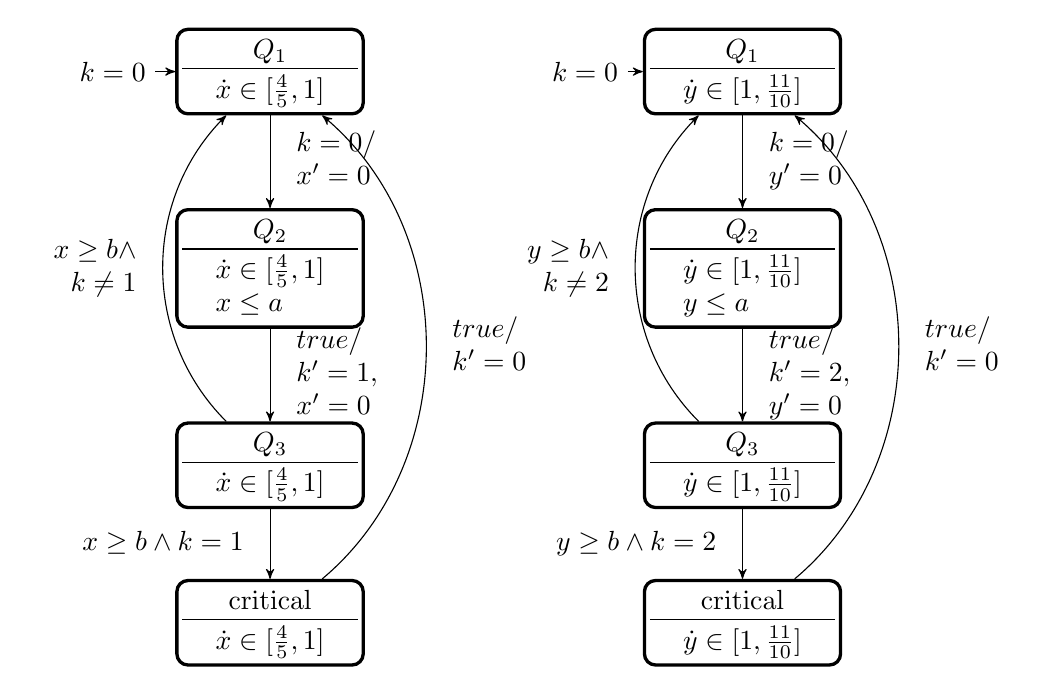
\begin{tikzpicture}[->,>=stealth']

    \begin{scope}
    \node[state] (Q1)
    {
      \begin{tabular}{c}
        $Q_1$ \\
        \hline \\[-1em]
        \begin{tabular}{l}
          $\dot{x} \in [\frac{4}{5},1]$ \\
        \end{tabular}
      \end{tabular}
    };
    
    \node[state,
    below of=Q1,
    node distance=2.5cm] (Q2)
    {
      \begin{tabular}{c}
        $Q_2$ \\
        \hline \\[-1em]
        \begin{tabular}{l}
          $\dot{x} \in [\frac{4}{5},1]$ \\
          $x \leq a$ 
        \end{tabular}
      \end{tabular}
    };

    \node[state,
    below of=Q2,
    node distance=2.5cm] (Q3)
    {
      \begin{tabular}{c}
        $Q_3$ \\
        \hline \\[-1em]
        \begin{tabular}{l}
          $\dot{x} \in [\frac{4}{5},1]$ \\
        \end{tabular}
      \end{tabular}
    };

    \node[state,
    below of=Q3,
    node distance=2cm] (CS)
    {
      \begin{tabular}{c}
        critical \\
        \hline \\[-1em]
        \begin{tabular}{l}
          $\dot{x} \in [\frac{4}{5},1]$ \\
        \end{tabular}
      \end{tabular}
    };

    \node[left of=Q1, node distance=2 cm] (INIT) {
      $k = 0$
    };

    \path
    (INIT) edge (Q1)

    (Q1)  edge node[anchor=left,right]
    {
      \begin{tabular}{l}
        $k = 0 /$ \\
        $x' = 0$
      \end{tabular}
    } (Q2)
    
    (Q2) edge node[anchor=left,right]
    {
      \begin{tabular}{l}
        $true /$ \\
        $k' = 1,$\\
        $x' = 0$
      \end{tabular}
    } (Q3)

    (Q3)  edge[bend left=45] node[anchor=right,left]
    {
      \begin{tabular}{r}
        $x \geq b \wedge$\\
        $k \neq 1$ \\
      \end{tabular}
    } (Q1)

    (Q3)  edge node[anchor=right,left]
    {
      \begin{tabular}{r}
        $x \geq b \wedge k = 1$ \\
      \end{tabular}
    } (CS)

    (CS)  edge[bend right=50] node[anchor=left,right]
    {
      \begin{tabular}{l}
        $true /$\\
        $k' = 0$
      \end{tabular}
    } (Q1);
  \end{scope}

  \begin{scope}[xshift=6cm]
    \node[state] (Q1)
    {
      \begin{tabular}{c}
        $Q_1$ \\
        \hline \\[-1em]
        \begin{tabular}{l}
          $\dot{y} \in [1,\frac{11}{10}]$ \\
        \end{tabular}
      \end{tabular}
    };
    
    \node[state,
    below of=Q1,
    node distance=2.5cm] (Q2)
    {
      \begin{tabular}{c}
        $Q_2$ \\
        \hline \\[-1em]
        \begin{tabular}{l}
          $\dot{y} \in [1,\frac{11}{10}]$ \\
          $y \leq a$ 
        \end{tabular}
      \end{tabular}
    };

    \node[state,
    below of=Q2,
    node distance=2.5cm] (Q3)
    {
      \begin{tabular}{c}
        $Q_3$ \\
        \hline \\[-1em]
        \begin{tabular}{l}
          $\dot{y} \in [1,\frac{11}{10}]$ \\
        \end{tabular}
      \end{tabular}
    };

    \node[state,
    below of=Q3,
    node distance=2cm] (CS)
    {
      \begin{tabular}{c}
        critical \\
        \hline \\[-1em]
        \begin{tabular}{l}
          $\dot{y} \in [1,\frac{11}{10}]$ \\
        \end{tabular}
      \end{tabular}
    };

    \node[left of=Q1, node distance=2 cm] (INIT) {
      $k = 0$
    };

    \path
    (INIT) edge (Q1)

    (Q1)  edge node[anchor=left,right]
    {
      \begin{tabular}{l}
        $k = 0 /$ \\
        $y' = 0$
      \end{tabular}
    } (Q2)
    
    (Q2) edge node[anchor=left,right]
    {
      \begin{tabular}{l}
        $true /$ \\
        $k' = 2,$\\
        $y' = 0$
      \end{tabular}
    } (Q3)

    (Q3)  edge[bend left=45] node[anchor=right,left]
    {
      \begin{tabular}{r}
        $y \geq b \wedge$\\
        $k \neq 2$ \\
      \end{tabular}
    } (Q1)

    (Q3)  edge node[anchor=right,left]
    {
      \begin{tabular}{r}
        $y \geq b \wedge k = 2$ \\
      \end{tabular}
    } (CS)

    (CS)  edge[bend right=50] node[anchor=left,right]
    {
      \begin{tabular}{l}
        $true /$\\
        $k' = 0$
      \end{tabular}
    } (Q1);
  \end{scope}

  \end{tikzpicture}
  \caption{Fischer mutual exclusion protocol}\label{fig:fischer}
\end{figure}

\figurename~\ref{fig:fischer} shows an instantiation of the Fischer
protocol for two processes, where $P_1$ has a relative clock speed
between $\frac{4}{5}$ and $1$, and $P_2$ has a relative clock speed
between $1$ and $\frac{11}{10}$. In general, a high value for $b$ will
guarantee that all concurrent writes will be finished before a process
checks variable $k$ and eventually enters the critical section. For
the given instantiation, it can be verified that for a maximum write
delay set to the unit value $a=1$, the choice of $b=2$ is sufficient
to guarantee a correct behavior. 

For performance reasons, a value as small as possible should be
chosen.  Starting the Inverse Method with the above instantiation
$\pi_0 = (1,2)$, the following constraint is derived:
\begin{equation}\label{eq:fischer}
  a \geq 0 \quad \wedge \quad b > \frac{11}{8} a
\end{equation}

This means that for any parameter instantiation satisfying
(\ref{eq:fischer}), the system will show the same discrete
behavior. Since the correctness of the protocol has been shown for
$\pi_0$, we can conclude that (\ref{eq:fischer}) is sufficient for the
mutual exclusion. The same result is obtained by performing a complete
parametric reachability analysis -- e.g.~with HyTech~\cite{HHW:97} --
and projecting the reachable states on the parameters. This also means
that the constraint generated by the inverse method is maximal.

\subsection{Water Tank Benchmark}

\begin{figure}[tb]
  \centering
  \small
  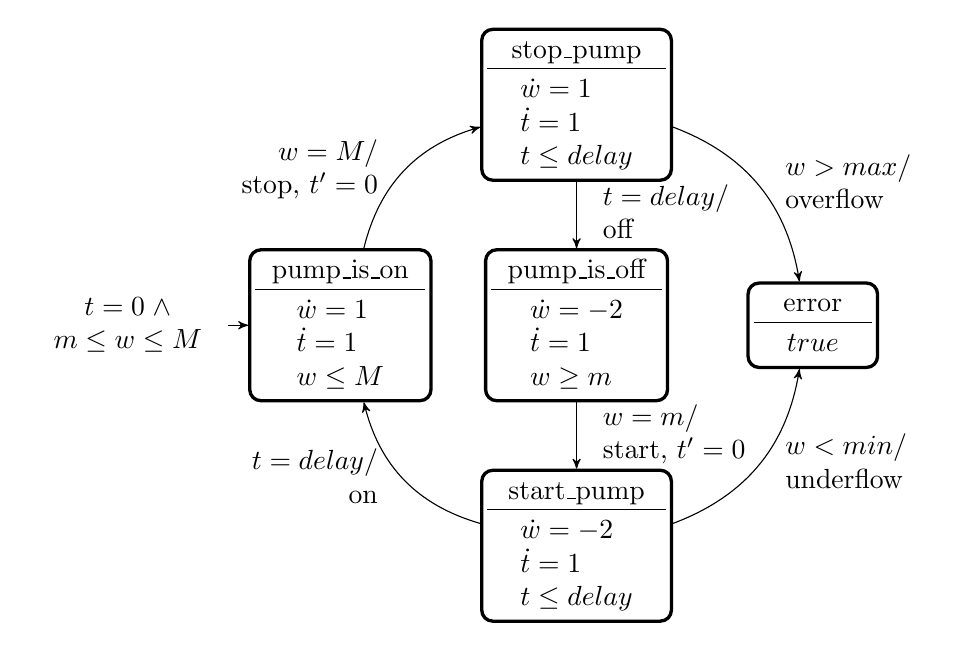
\begin{tikzpicture}[->,>=stealth']

    \node[state] (ON)
    {
      \begin{tabular}{c}
        pump\_is\_on \\
        \hline \\[-1em]
        \begin{tabular}{l}
          $\dot{w} = 1$ \\
          $\dot{t} = 1$ \\
          $w \leq M$
        \end{tabular}
      \end{tabular}
    };
    
    \node[state,
    right of=ON,
    node distance=3cm] (OFF)
    {
      \begin{tabular}{c}
        pump\_is\_off \\
        \hline \\[-1em]
        \begin{tabular}{l}
          $\dot{w} = -2$ \\
          $\dot{t} = 1$ \\
          $w \geq m$
        \end{tabular}
      \end{tabular}
    };

    \node[state,
    above of=OFF,
    node distance=2.8cm] (STOP)
    {
      \begin{tabular}{c}
        stop\_pump \\
        \hline \\[-1em]
        \begin{tabular}{l}
          $\dot{w} = 1$ \\
          $\dot{t} = 1$ \\
          $t \leq delay$
        \end{tabular}
      \end{tabular}
    };

    \node[state,
    below of=OFF,
    node distance=2.8cm] (START)
    {
      \begin{tabular}{c}
        start\_pump \\
        \hline \\[-1em]
        \begin{tabular}{l}
          $\dot{w} = -2$ \\
          $\dot{t} = 1$ \\
          $t \leq delay$
        \end{tabular}
      \end{tabular}
    };

    \node[state,
    right of=OFF,
    node distance=3cm] (ERROR)
    {
      \begin{tabular}{c}
        error \\
        \hline \\[-1em]
        \begin{tabular}{l}
          $true$ \\
        \end{tabular}
      \end{tabular}
    };

    \node[left of=ON, node distance=2.7cm] (INIT) {
      \begin{tabular}{c}
        $t = 0 \; \wedge$\\
        $m \leq w \leq M$
      \end{tabular}
    };


    \path
    (INIT) edge (ON)

    (ON)  edge[bend left=30] node[anchor=right,left]
    {
      \begin{tabular}{r}
        $w = M /$ \\
        stop, $t' = 0$
      \end{tabular}
    } (STOP)
    
    (STOP) edge node[anchor=left,right]
    {
      \begin{tabular}{l}
        $t = delay /$ \\
        off
      \end{tabular}
    } (OFF)

    (OFF) edge node[anchor=left,right]
    {
      \begin{tabular}{l}
        $w = m /$\\
        start, $t' = 0$
      \end{tabular}
    } (START)

    (START)  edge[bend left=30] node[anchor=right,left]
    {
      \begin{tabular}{r}
        $t = delay /$ \\
        on
      \end{tabular}
    } (ON)

    (STOP)  edge[bend left=30] node[anchor=left,right]
    {
      \begin{tabular}{l}
        $w > max /$ \\
        overflow
      \end{tabular}
    } (ERROR)

    (START)  edge[bend right=30] node[anchor=left,right]
    {
      \begin{tabular}{l}
        $w < min /$ \\
        underflow
      \end{tabular}
    } (ERROR);

  \end{tikzpicture}
  \caption{LHA of a controlled water reservoir}\label{fig:aut1}
\end{figure}

\subsubsection{The Model} 
As another benchmark with a total number of five parameters, we consider
a monitored water reservoir \cite{HPR:97}, modeled by the LHA in
\figurename~\ref{fig:aut1}. The state variables are the water level $w$
and a global clock $t$. There is a pump attached to the reservoir,
providing it with fresh water. When the pump is on, the water level
increases with a constant rate of $\dot{w} = 1$. When it is off, the
reservoir is drained at a rate of $\dot{w} = -2$. As parameters, $max$
and $min$ give the bounds on $w$ that should be respected by the
system. $M$ and $m$ give limits on the water level for which the pump
is (de-) activated. But, there is a $delay$ needed to actually change
the activity of the pump. While waiting for the pump to react, an
$overflow$ ($w > max$) or $underflow$ ($w < min$) can happen, leading
the system to an error state.


\subsubsection{Inverse Method}
The inverse method can be used to derive appropriate constraints on
the parameters $min, max, M, m$ and $delay$ such that no overflow or
underflow can happen. A reference valuation $\pi_0$ can easily be
found for a short $delay$ and by allowing for sufficiently large
margins between $min$ and $m$ ($M$ and $max$), respectively. As
starting point, $\pi_0 = (min \mapsto 0, m \mapsto 10, M \mapsto 20,
max \mapsto 30, delay \mapsto 1)$ is used. As a result, the following
constraint is generated using forward
reachability\footnote{Additionally to the shown inequalities, only
  non-negative parameters are considered.}:
\begin{equation} \label{eq:tank_K0}
\begin{array}{rl}
  M + delay & \geq m \;\wedge\\
  m & \geq min + 2\cdot delay \;\wedge\\
  max & \geq M + delay
\end{array}
\end{equation}

\begin{figure}[tb]
  \centering
  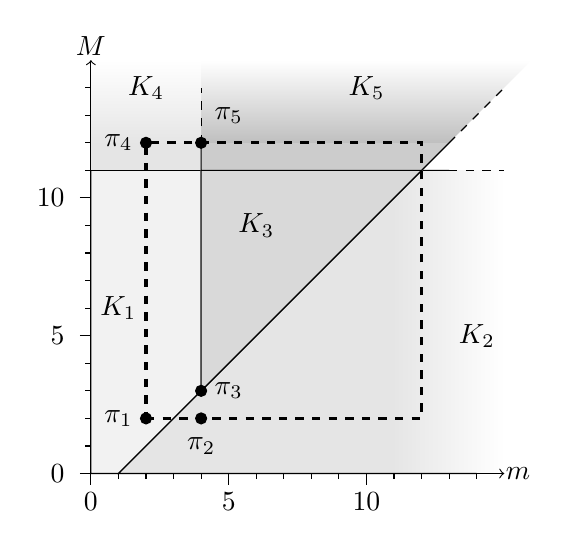
\begin{tikzpicture}[scale=0.35]
    % Z1
    \draw[fill=gray!10] (0,0) -- (1,0) -- (4,3) -- (4,11) -- (0,11) --cycle;
    
    % Z2 
    \draw[fill=gray!20, color=gray!20] (13,0) -- (1,0) -- (12,11) -- (13,11) -- cycle;
    \shade[right color=white,left color=gray!20] (11,0) -- (15,0) -- (15,11) -- (11,11) -- cycle;
    \draw (14,0) -- (1,0) -- (12,11) -- (13,11);
    
    % Z3
    \draw[fill=gray!30] (4,3) -- (12,11) -- (4,11) -- cycle;

    % Z4
    \draw[fill=gray!20,color=gray!20] (0,12) -- (0,11) -- (4,11) -- (4,12) -- cycle;
    \shade[bottom color=gray!20,top color=white] (0,15) -- (0,12) -- (4,12) -- (4,15) -- cycle;
    \draw (0,13) -- (0,11) -- (4,11) -- (4,12);
    
    % Z5
    \draw[fill=gray!40,color=gray!40] (4,12) -- (4,11) -- (12,11) -- (13,12) -- cycle;
    \shade[bottom color=gray!50,top color=white] (4,12) -- (4,15) -- (16,15) -- (13,12) -- cycle;

    \draw (4,12) -- (4,11) -- (12,11) -- (13,12);
    
    % V0
    \draw[very thick, dashed] (2,2) -- (12,2) -- (12,12) -- (2,12) -- cycle;
    
    % infinity directions
    \draw[dashed] (4,12) -- (4,14);
    \draw[dashed] (13,12) -- (15,14);
    \draw[dashed] (13,11) -- (15,11);

    % Zone names
    \draw (1,6) node {$K_1$};
    \draw (14,5) node {$K_2$};
    \draw (6,9) node {$K_3$};
    \draw (2,14) node {$K_4$};
    \draw (10,14) node {$K_5$};

    % Pis
    \draw[fill=black] (2,2) circle (0.2cm); \draw (1,2) node {$\pi_1$};
    \draw[fill=black] (4,2) circle (0.2cm); \draw (4,1) node {$\pi_2$};
    \draw[fill=black] (4,3) circle (0.2cm); \draw (5,3) node {$\pi_3$};
    \draw[fill=black] (2,12) circle (0.2cm); \draw (1,12) node {$\pi_4$};
    \draw[fill=black] (4,12) circle (0.2cm); \draw (5,13) node {$\pi_5$};

    % Boundary marks
    % \draw[-triangle 90 reversed, line width=0pt] (4.1,7) -- (4,7);
    % \draw[-triangle 90 reversed, line width=0pt] (8,10.9) -- (8,11);
    % \draw[-triangle 90 reversed, line width=0pt] (7.9,7.1) -- (8,7);

    % axes
    \draw[->] (0,0) -> ++(15,0);
    \draw[->] (0,0) -> ++(0,15);
    \draw (15.5,0) node {$m$};
    \draw (0,15.5) node {$M$};

    %% tics
    \foreach \x in {0,1,...,14} \draw (\x,-0.2) -- (\x,0);
    \foreach \y in {0,1,...,14} \draw (-0.2,\y) -- (0,\y);
    
    \foreach \x in {0,5,10} \draw (\x,-0.4) -- (\x,0);
    \foreach \x in {0,5,10} \draw (\x,-1) node {\x};

    \foreach \y in {0,5,10} \draw (-0.4,\y) -- (0,\y);
    \foreach \y in {0,5,10} \draw (-0.6,\y) node[left] {\y};
  \end{tikzpicture}

  \caption{Cartography for water reservoir}\label{fig:cart}
\end{figure}


\subsubsection{Behavioral Cartography}
In order to fully explore the possible behaviors of the system, the
cartography algorithm is applied, with varying parameters $m$ and
$M$. The remaining parameters are fixed to the values $min = 2, max =
12$ and $delay = 1$. The zone to explore is given by the interval $m,M
\in [min,max]$. 

The cartography results in five different tiles, shown in
\figurename~\ref{fig:cart}. In the figure also the starting points $\pi_1$
to $\pi_5$ can be found, that were used to call the Inverse Method. As
it turns out, the whole (real-valued) rectangle $[2, 12]^2$ is covered
by the generated constraints. Furthermore, the trace set associated
with constraint $K_3$ is the only one that corresponds to a good
behavior of the system. Thus, the constraint in (\ref{eq:tank_K0}) is
maximal. 

\subsection{Navigation Benchmark} \label{sec:nav}
\subsubsection{The Model}
The \emph{navigation benchmark} has been described in
\cite{FI:2004}. It describes an object moving in a plane. The plane is
divided into square fields, where each field is associated with one of
eight directions, to which the movement of the object
converges. Furthermore, there are bad fields (marked $B$) that need to
be avoided and good fields (marked $A$) that should eventually be
reached by the object.

\begin{figure}[t]
  \centering
  \subfigure[Reachable states from point]{
    \includegraphics[width=5cm]{images/navigation_map.pdf}
    \label{fig:nav}
  }
  \hfill
  \subfigure[Behavioral cartography]{
    \includegraphics[width=5cm]{images/navigation_cart.pdf}
    \label{fig:navcart}  
  }
  \caption{Navigation benchmark}
\end{figure}

More formally, the object has the current position $(x, y)^T$. The
horizontal and vertical velocity are described by the vector $v =
(v_x, v_y)^T$. For each field in the matrix $F$, the desired velocity
is given as $v_{d} = (sin(i \cdot \pi /4), \, cos(i \cdot \pi /
4))^T$, with a given $i \in \{0,\dots,7\}$. The convergence of the current
velocities to the desired ones is determined by the differential
equation $\dot{v} = A(v - v_d)$, where the matrix $A \in
\Reals^{2\times 2}$ is given by the benchmark instance. For example,
\figurename~\ref{fig:nav} shows a $3\times 3$ benchmark instance given by
\begin{equation}\label{eq:nav}
  F = \left(
  \begin{matrix}
    B & 2 & 4 \\
    2 & 2 & 4 \\
    1 & 1 & A \\
  \end{matrix}
  \right), \;
  A = \left(
    \begin{matrix}
      -1.2 & 0.1 \\
      0.1 & -1.2 \\
    \end{matrix}
  \right),
\end{equation}
with the initial states defined as $x \in [0,1], y \in [0,1], v_x \in
[0.1, 0.5]$ and $v_y \in [0.05, 0.25]$.

The system can be modeled by an AHA in a straightforward way, where
each field corresponds to a control location. In order to compute the
reachable states, the system needs to be linearized wrt.~variables
$v_x, v_y$. The initial states are represented by parameters $x_0,
y_0, v_{x0}, v_{y0}$.

\subsubsection{Behavioral Cartography}
While a full parametric reachability analysis is costly, the system
can be analyzed point-wise. This means that the parameters defining
the initial state are fixed to a single value, while the behavioral
cartography is used to obtain a measure of coverage of the verified
behavior. As an example, the blue regions in \figurename~\ref{fig:nav}
represent the reachable states from the initial point $(0.5, 0.5)^T$.

In an experiment, we explore the parameter space for the two
parameters $x_0, y_0$ within the interval $[0,1]$ with a step size
$\delta = 0.1$. In this way, we obtain eight different tiles, that
almost completely cover the considered rectangle, see
\figurename~\ref{fig:navcart}. Only a small triangular region on the right
hand side of the figure remains uncovered. All the covered tiles are
classified as good tiles, since the bad state is not reached. 

\subsubsection{Coverage}
Another instance of the navigation benchmark is considered in
\cite{JFG+:2007}, given by the map
\begin{equation}
  F = \left(
  \begin{matrix}
    B & 2 & 4 \\
    4 & 3 & 4 \\
    2 & 2 & A \\
  \end{matrix}
  \right)
\end{equation}
and the matrix $A$ as in \eqref{eq:nav}. There, the coverage of the
initial states in the rectangle $[1,2] \times [1,2]$ with $v_{x0} =
-0.2$ and $v_{y0} = 0$ is computed, starting with 25 equally
distributed test points. The computed coverage is reported with $48
\%$. In contrast, using the behavioral cartography, only a coverage of
more that $97 \%$ is achieved with only 9 different tiles\footnote{Two
  of the tiles degenerate to a point or a line and can thus not be
  seen in the figure}, as depicted in \figurename~\ref{fig:navcart2}.

\begin{figure}[tb]
  \centering
  \includegraphics[width=5cm]{images/navigation_cart2.pdf}
  \caption{Coverage of initial states}
  \label{fig:navcart2}    
\end{figure}

For the same map, the initial states $(x,y)^T \in [2.2,2.8] \times
[1.2,1.8]$ were considered. Starting with 9 test points, an estimated
coverage of $72 \%$ was computed. In constrast, choosing any single
point in the given initial region, a single constraint is generated by
the inverse method, which covers $100 \%$ of the rectangle. 


%%%%%%%%%%%%%%%%%%%%%%%%%%%%%%%%%%%%%%%%%%%%%%%%%%%%%%%%%%%%%%%%%%%%%%%%%%%%
\section{Discussion}\label{sec:disc}
% - extension to LHA straight-forward
% - problems due to static linearization
% - resolved by grouping states
% - expensive analysis
% - but trade-offs possible

As shown in the previous sections, the inverse method -- having been
introduced for the analysis of timed automata -- can be applied as
well for hybrid systems. The extension to automata with rectangular
and linear dynamics is straightforward, using the relation between
concrete and symbolic semantics which extends nicely to these classes
of hybrid automata. However, almost all non-trivial examples of hybrid
systems from the literature have affine dynamics. The naive approach
-- approximating affine models statically by LHA -- shows limited
results, as the partitioning of locations leads to a great number of
distinct trace sets.

Instead, the partitioning can be applied locally, incorporating it
into the time-elapse operator and thereby grouping states that belong
to the same location of the original affine model. In this way, more
general constraints and thus a better coverage can be achieved. The
additional convex hull operation can however be quite costly and
strongly depends on the chosen number of partitions per
dimension. This can be seen as a trade-off between precision and
performance of the analysis. In practice, the method can be applied in
an iterative manner, starting with a very coarse linearization, and
then concentrating on small parts of the parameter space with a finer
approximation.

The presented methods rely only on trace sets, abstracting from the
valuations of the continuous variables. For this reason they are best
suited for the verification of qualitative properties, like the
(non-)reachability of a set of locations. Since many interesting
properties -- like safety conditions -- can be expressed as
reachability, this is not a serious limitation. There are also
quantitative properties that can be coded as reachability, e.g.~by
adding a transition to a bad state when a certain deadline or
threshold value is violated. Also for this class of properties, our
methods can be applied.

%%%%%%%%%%%%%%%%%%%%%%%%%%%%%%%%%%%%%%%%%%%%%%%%%%%%%%%%%%%%%%%%%%%%%%%%%%%%
\section{Conclusions}\label{sec:concl}
In this report, we present a method to derive parameter constraints
for LHA, that guarantee the same behavior as for a reference valuation
of the parameters. This inverse method has been recently introduced
for deriving timing constraints for timed automata. Here, we provide
the extension of the method to LHA. Furthermore, it is shown how the
reachability procedure can be adapted to enable the analysis of
systems with affine dynamics. 

The method can be used to attack the parameter synthesis problem for
LHA, by generalizing a reference valuation that is known to guarantee
a good behavior. By early pruning of invalid states, the method is
more efficient than the parameter synthesis based on standard
reachability analysis.  Repeated analysis for different starting
points yields a ``behavioral cartography''. This allows to cover
large parts of the initial state space of nondeterministic hybrid
systems, thus providing an alternative tool to the symbolic simulation
method of \cite{AKRS:2008}.

The extended algorithms have been implemented in the tool
IMITATOR. The tool has been demonstrated on a hybrid system benchmark,
a distributed temperature control system. While standard
parameterized reachability analysis fails, a good coverage of the
parameter space can be achieved with our method.


%%%%%%%%%%%%%%%%%%%%%%%%%%%%%%%%%%%%%%%%%%%%%%%%%%%%%%%%%%%%%%%%%%%%%%%%%%%%
\bibliographystyle{abbrv}
\bibliography{litbank}

\appendix
\clearpage

%%%%%%%%%%%%%%%%%%%%%%%%%%%%%%%%%%%%%%%%%%%%%%%%%%%%%%%%%%%%%%%%%%%%%%%%%%%%

% \section{Proofs}

% In order to prove the correctness of the formal verification methods
% which are based on the symbolic semantics, we establish a relation
% between the concrete and the symbolic semantics. More precisely, we
% show that every concrete run can be simulated by a symbolic run and
% vice versa. The following statements are motivated by
% \cite{HRSV:2001}, adapting their proofs to the LHA model.



% Based on these lemmata, we give a proof of Proposition~\ref{prop:run_sc}.



% \begin{lemma}\label{lem:step_cs}
%   For each step $(q,w) \Trans{a} (q',w')$ in the concrete semantics of
%   $\A[\pi]$, there is a step $(q,C) \Trans{a} (q',C')$ in the
%   symbolic semantics of $\A(K)$ for some parameter constraint
%   $K$ and $\left<w', \pi\right> \models C'$.
% \end{lemma}

% \begin{proof}
%   The concrete step $(q,w) \Trans{a} (q',w')$ consists of the two
%   steps $(q,w) \trans{a} (q',w'') \trans{t} (q',w')$.

%   For the delay transition, we have $\exists r \in D_{q'}, d \in
%   \Reals_{+}: w' = w'' + d \cdot r$ and $\left<w', \pi\right>
%   \models C'$. Thus there exists a region $C''$ with
%   $\left<w'',\pi\right> \models C''$ and $\left<w', \pi\right>
%   \models C'' \elapse D_{q'}$.
    

%   \qed
% \end{proof}

% In the following, we give a proof of Proposition~\ref{prop:run_cs}.

% \section{Correctness of algorithm \IM}
% \label{app:IM}

% [\dots]

% Suppose $\IM(\A, \pi_0)$ terminates with output $K_0$. Let $K$ be the
% current constraint on parameters, and $S$ the set of reachable
% states. We have $S = Reach_{\A(K)}$ and $K_0 = \bigcap_{(q,C)\in
%   S}(\exists X:C)$.

% \begin{lemma}
%   We have $K_0 \subseteq K$.
% \end{lemma}
% \begin{proof}
%   With Lemma~\ref{lem:narrow}, for each state $(q,C) \in S$ it holds
%   that $(\exists X:C) \subseteq K$. This implies that also $K_0 =
%   \bigcap_{(q,C)\in S}(\exists X:C) \subseteq K$. \qed
% \end{proof}

% \begin{lemma}
%   We have $\pi_0 \models K_0$.
% \end{lemma}
% \begin{proof}
%   When \IM terminates, all states are $\pi_0$-compatible, i.e.~$\pi_0
%   \models (\exists X:C)$ for all $(q,C) \in S$. Thus, also the
%   intersection $K_0$ of these constraints must satisfy $\pi_0$. \qed
% \end{proof}

% \begin{lemma}
%   For all $\pi$ with $\pi \models K_0$, for all symbolic runs of
%   $\A(K)$ reaching $(q,C)$, there exists a clock valuation $w$ such
%   that $\left<w, \pi\right> \models C$. 
% \end{lemma}
% \begin{proof}
%   For all symbolic run of $\A(K)$, we have $(q,C) \in S$, since $S =
%   Reach_{\A(K)}({s_0})$. Moreover, we have $K_0 = \bigcap_{(q,C)\in
%     S}(\exists X:C)$. 
% \end{proof}

%%%%%%%%%%%%%%%%%%%%%%%%%%%%%%%%%%%%%%%%%%%%%%%%%%%%%%%%%%%%%%%%%%%%%%%%%%%%


%% \clearpage
\section{Notational Conventions}

\begin{tabular}{ll}
  $a$ & action \\
  $g$ & guard \\
  $i,j$ & index \\
  $m,n$ & natural number \\
  $p$ & parameter \\
  $q$ & location \\
  $s$ & state \\
  $t$ & real number \\
  $u,v,w$ & valuation (point) \\
  $x,y$ & continuous variable \\
  
  $C$ & constraint \\
  $D$ & flow constraint (convex set of time derivatives) \\
  $I$ & invariant \\
  $K$ & parameter constraint \\
  $M$ & total number of parameters \\
  $N$ & total number of clocks \\  
  $P$ & set of parameters \\
  $Q$ & set of locations \\
  $R$ & run \\
  $S$ & set of states \\
  $T$ & trace \\
  $X$ & set of continuous variables \\
  $Z$ & set of parameter constraints \\

  $\alpha, \beta$ & integers \\
  $\delta$ & step size for behavioral cartography\\
  $\mu$ & jump relation \\
  $\pi$ & parameter valuation (point) \\
  $\Sigma$ & alphabet \\

  $\A$ & parametric linear hybrid automaton \\
  $\mathcal{L}$ & set of convex linear constraints \\
  $\valuation$ & set of valuations \\

  $\Naturals$ & the natural numbers \\
  $\Ints$ & the integers \\
  $\Reals$ & the real numbers
\end{tabular}

% \section{Illustrative Example} \label{sec:example} Consider the
% automaton in \figurename~\ref{fig:simple_aut}.  The two transitions
% from the initial state are guarded by constraints over the parameter
% $p$. Given the parameter constraint $K \Leftrightarrow 1 \leq p \leq
% 2$, the traces contained in the symbolic semantics of $\A(K)$ are
% shown in \figurename~\ref{fig:trace_k}, while the concrete semantics
% for the parameter valuations $\pi_1 = (p \mapsto 1)$ and $\pi_2 = (p
% \mapsto 2)$ are depicted in \figurenames~\ref{fig:trace_pi1} and
% \ref{fig:trace_pi2}, respectively. Note that in this case, the traces
% of $\A(K)$ are the union of the traces of $\A[\pi_1]$ and
% $\A[\pi_2]$. There is a constraint $K_1 \Leftrightarrow p < 2$ (and
% $K_2 \Leftrightarrow p \geq 2$), such that $\A(K_1)$ and $\A[\pi_1]$
% (resp.~$\A(K_2)$ and $\A[\pi_2]$) are trace equivalent.
% \begin{figure}[tb]
%   \centering

%   \small
%   \begin{tikzpicture}[->,>=stealth']

%     \node[state] (Q0)
%     {
%       \begin{tabular}{c}
%         $Q_0$\\
%         \hline
%         $true$
%       \end{tabular}
%     };

%     \node[left of=Q0, node distance=1cm] (INIT) {} ;
    
%     \node[state] (Q1) at (3,1)
%     {
%       \begin{tabular}{c}
%         $Q_1$\\
%         \hline
%         $true$
%       \end{tabular}
%     };

%     \node[state] (Q2) at (3,-1)
%     {
%       \begin{tabular}{c}
%         $Q_2$\\
%         \hline
%         $true$
%       \end{tabular}
%     };

%     \path
%     (INIT) edge (Q0)
    
%     (Q0) edge [bend left=20,above] node
%     {
%       $p < 2 \; / \; a$
%     } (Q1)

%     (Q0) edge [bend right=20,below] node
%     {
%       $p \geq 2 \; / \; b$
%     } (Q2);
%   \end{tikzpicture}
%   \caption{Simple automaton $\A$}\label{fig:simple_aut}
% \end{figure}

% \begin{figure}[tb]
%   \centering

%   \subfigure[Traces of $\A(K)$\label{fig:trace_k}]{
%     \small
%     \begin{tikzpicture}[->,>=stealth']
%       \node[location]           (Q0) {$Q_0$};
%       \node[location] at (2,0.7)  (Q1) {$Q_1$};
%       \node[location] at (2,-0.7) (Q2) {$Q_2$};

%       \path
%       (Q0) edge [double, above] node {$a$} (Q1)
%       (Q0) edge [double, below] node {$b$} (Q2);
%     \end{tikzpicture}  
%   }
%   \hfill
%   \subfigure[Traces of {$\A[\pi_1]$}\label{fig:trace_pi1}]{
%     \small
%     \begin{tikzpicture}[->,>=stealth',baseline=-2]      
%       \node[location] (Q0) at (0,1) {$Q_0$};
%       \node[location] (Q1) at (2,1) {$Q_1$};

%       \path
%       (Q0) edge [double, above] node {$a$} (Q1);
%     \end{tikzpicture}  
%   }
%   \hfill
%   \subfigure[Traces of {$\A[\pi_2]$}\label{fig:trace_pi2}]{
%     \small
%     \begin{tikzpicture}[->,>=stealth',baseline=-2]
%       \node[location] (Q0) at (0,1) {$Q_0$};
%       \node[location] (Q2) at (2,1) {$Q_2$};

%       \path
%       (Q0) edge [double, above] node {$b$} (Q2);
%     \end{tikzpicture}  
%   }
%   \caption{Traces for symbolic and concrete semantics of
%     $\A$}\label{fig:traces}
% \end{figure}

\end{document}

